\documentclass[a4paper,twoside]{memoir}
% Set up encoding
\usepackage[utf8]{inputenc}

% Mulighed for at definere acronyms
\usepackage{acronym}

% Load up bibliography.
\usepackage[authoryear]{natbib}
\setcitestyle{numbers,square}
% Bibliography style.
\bibliographystyle{plainnat}

% Algorithm support.
\usepackage{algorithmic}
\usepackage{algorithm}
\usepackage{subfig}
\usepackage{amsmath}
\usepackage{amsfonts}
% Make algorithms appear as procedures instead.
\floatname{algorithm}{Procedure}
\renewcommand{\algorithmicrequire}{\textbf{Input:}}
\renewcommand{\algorithmicensure}{\textbf{Output:}}

% Image frames.
\setlength{\fboxsep}{0pt}
\setlength{\fboxrule}{0.5pt}

% Also, images.
\usepackage{graphicx}

% tabeller der strækker sig over flere sider
\usepackage{longtable}

% flere tabel-muligheder
\usepackage{multirow}

% bedre enumerate
\usepackage{enumitem}

% Mulighed for if-then-else sætning!
\usepackage{ifthen}

% Todo notes here and there.
% write instead for disable: \usepackage[disable]{todonotes}
\usepackage{todonotes}

% Forbedrede floats.
\usepackage{float}
\usepackage{rotating}

\newsubfloat{figure}

% Special symbols availability.
\usepackage{amssymb}

%Degree symbol
\usepackage{gensymb}

% Wrap figure
\usepackage{wrapfig}

%landscape mode
\usepackage{lscape}

\usepackage{booktabs}
\usepackage{hvfloat}
\usepackage{units}

%Fun with captions
\usepackage{caption}


% Neat-o referencer...o.
\usepackage{bookmark,hyperref}
\usepackage{nameref}

\newcommand{\secref}[1]{Section \ref{#1}}
\newcommand{\chapref}[1]{Chapter \ref{#1}}
\newcommand{\appref}[1]{Appendix \ref{#1}}

% Skriver Appendix foran Appendices
\renewcommand*{\cftpartname}{PART~}
%\renewcommand*{\cftchaptername}{\chaptername~}
\renewcommand*{\cftappendixname}{\appendixname~}
%\renewcommand*{\cftchapteraftersnum}{.}% dot after the number
%\setlength{\cftchapternumwidth}{2em}

% Operationel semantik
\newcommand{\lag}{\langle}
\newcommand{\rag}{\rangle}
\newcommand{\setof}[2]{\ensuremath{\{ #1 \mid #2 \}}}
\newcommand{\set}[1]{\ensuremath{\{ #1 \}}}
\newcommand{\besk}[1]{\ensuremath{\lag #1 \rag}}
\newcommand{\ra}{\rightarrow}
\newcommand{\lra}{\longrightarrow}
\newcommand{\Ra}{\Rightarrow}

% CODE %
\usepackage{listings}
\usepackage{color}
%\usepackage{bera}
\definecolor{gray}{rgb}{0.4,0.4,0.4}
\definecolor{darkblue}{rgb}{0.0,0.0,0.6}
\definecolor{cyan}{rgb}{0.0,0.6,0.6}
\definecolor{dkgreen}{rgb}{0,.6,0}
\definecolor{dkblue}{rgb}{0,0,.6}
\definecolor{dkyellow}{cmyk}{0,0,.8,.3}

\lstset{
  basicstyle=\ttfamily,
  columns=fullflexible,
  showstringspaces=false,
  commentstyle=\color{gray}\upshape,
  basicstyle=\small,
  numberstyle=\footnotesize,
  numbers=left,
  captionpos=b,
  stepnumber=1,
  numbersep=10pt,
  tabsize=2,
  breaklines=true,
}
% Define markup of XML
\lstdefinelanguage{XML}
{
  morestring=[b]",
  morestring=[s]{>}{<},
  morecomment=[s]{<?}{?>},
  identifierstyle=\color{darkblue},
  keywordstyle=\color{cyan},
  morekeywords={id, target, type, category, value, point, correct, rows, width, time}% list your attributes here
}
% Define markup of C#
\lstdefinelanguage{CSharp}[Visual]{C++}
{
	identifierstyle=\color{darkblue},
	commentstyle=\color{green!70!black}\itshape ,
	stringstyle=\color{gray},
	sensitive=true,
	morestring=[b]",
	morestring=[b]',
	morecomment=[l]//,
	morecomment=[n]{/*}{*/}
}

% Define markup of Javascript
\lstdefinelanguage{JavaScript}{
  keywords={typeof, new, true, false, catch, function, return, null, catch, switch, var, if, in, while, do, else, case, break},
  keywordstyle=\color{blue}\bfseries,
  ndkeywords={class, export, boolean, throw, implements, import, this},
  ndkeywordstyle=\color{darkgray}\bfseries,
  identifierstyle=\color{black},
  sensitive=false,
  comment=[l]{//},
  morecomment=[s]{/*}{*/},
  commentstyle=\color{purple}\ttfamily,
  stringstyle=\color{red}\ttfamily,
  morestring=[b]',
  morestring=[b]"
}

% Define markup of Java
\definecolor{dkgreen}{rgb}{0,0.6,0}
\definecolor{gray}{rgb}{0.5,0.5,0.5}
\definecolor{mauve}{rgb}{0.58,0,0.82}
\definecolor{keywordpurple}{RGB}{145, 0, 109}
\definecolor{background}{RGB}{240, 240, 240}
 
\lstset{
  language=java,
  %basicstyle=\footnotesize,       % the size of the fonts that are used for the code
  numbers=left,                   % where to put the line-numbers
  numberstyle=\tiny\color{black},  % the style that is used for the line-numbers
  stepnumber=1,                   % the step between two line-numbers. If it's 1, each line will be numbered 
  numbersep=5pt,                  % how far the line-numbers are from the code
  backgroundcolor=\color{background},  % choose the background color. You must add \usepackage{color}
  showspaces=false,               % show spaces adding particular underscores
  showstringspaces=false,         % underline spaces within strings
  showtabs=false,                 % show tabs within strings adding particular underscores
  frame=single,                   % adds a frame around the code
  rulecolor=\color{black},        % if not set, the frame-color may be changed on line-breaks within not-black text (e.g. comments (green here))
  tabsize=4,                      % sets default tabsize to 4 spaces
  captionpos=b,                   % sets the caption-position to bottom
  breaklines=true,                % sets automatic line breaking
  breakatwhitespace=false,        % sets if automatic breaks should only happen at whitespace
  title=\lstname,                 % show the filename of files included with \lstinputlisting;
                                  % also try caption instead of title
  keywordstyle=\color{keywordpurple}\bfseries,      % keyword style
  commentstyle=\color{dkgreen},   % comment style
  stringstyle=\color{blue},      % string literal style
  escapeinside={\%*}{*)},         % if you want to add a comment within your code
  morekeywords={*,...},           % if you want to add more keywords to the set
  morecomment=[l]//               % set // to register as a comment (for a line)
}

% Define markup of JSON
\colorlet{punct}{red!60!black}
\colorlet{delim}{red!60!black}
\colorlet{numb}{magenta!60!black}
\lstdefinelanguage{json}{
    basicstyle=\footnotesize,
    numbers=left,
    numberstyle=\tiny\color{black},
    identifierstyle=\color{dkgreen},
    stepnumber=1,
    numbersep=5pt,
    showspaces=false,
    showstringspaces=false,
    showtabs=false,
    breaklines=true,
    breakatwhitespace=false,
    tabsize=4,
    rulecolor=\color{black},
    captionpos=b,
    title=\lstname,
    frame=single,
    backgroundcolor=\color{background},
    literate=
     *{0}{{{\color{numb}0}}}{1}
      {1}{{{\color{numb}1}}}{1}
      {2}{{{\color{numb}2}}}{1}
      {3}{{{\color{numb}3}}}{1}
      {4}{{{\color{numb}4}}}{1}
      {5}{{{\color{numb}5}}}{1}
      {6}{{{\color{numb}6}}}{1}
      {7}{{{\color{numb}7}}}{1}
      {8}{{{\color{numb}8}}}{1}
      {9}{{{\color{numb}9}}}{1}
      {:}{{{\color{punct}{:}}}}{1}
      {,}{{{\color{punct}{,}}}}{1}
      {\{}{{{\color{delim}{\{}}}}{1}
      {\}}{{{\color{delim}{\}}}}}{1}
      {[}{{{\color{delim}{[}}}}{1}
      {]}{{{\color{delim}{]}}}}{1},
}

\lstdefinelanguage{phpstyle}{
  language        = php,
  keywordstyle    = \color{dkblue},
  morekeywords    = {function},
  stringstyle     = \color{red}
  }

\lstdefinelanguage{KAPAOOW}{
 sensitive=false,
 keywords={character, characters, action, end, if, then, else, from, to, downto, next, while, loop, use, turn, begins, ends, select, wins, draw, random, of, case, cases, enemy, player, start, skip, attack, types, damage, defend, by, using, message, and, or, is, value, mod},
 identifierstyle=\itshape,
 keywordstyle=\bfseries,
 stringstyle=\normalfont,
 morestring=[b]",
 comment=[l]{//},
 commentstyle=\color{gray}
}

% hack fra nettet.
% http://tex.stackexchange.com/questions/1230/reference-name-of-description-list-item-in-latex
\makeatletter
\let\orgdescriptionlabel\descriptionlabel
\renewcommand*{\descriptionlabel}[1]{
  \let\orglabel\label
  \let\label\@gobble
  \phantomsection
  \edef\@currentlabel{#1}
  %\edef\@currentlabelname{#1}
%  \let\label\orglabel
  \orgdescriptionlabel{#1}
}
\makeatother
% Rettehak. Meget lettere end \checkmark
\newcommand{\yes}{\checkmark}


% Create a new command, HRule, to insert some nice horisontal rules on the title page.
\newcommand{\HRule}{\rule{\linewidth}{0.3mm}}

% New command for two figures, side by side.
\newcommand{\twofigs}[6]
{
	\begin{figure}[H]
		\begin{minipage}[b]{0.5\columnwidth}
		\centering
		\includegraphics[width=0.8\columnwidth]{img/#1}
		\caption{#2\label{#3}}
		\end{minipage}
		\hspace{0.5cm}
		\begin{minipage}[b]{0.5\columnwidth}
		\centering
		\includegraphics[width=0.8\columnwidth]{img/#4}
		\caption{#5\label{#6}}
		\end{minipage}
	\end{figure}
}

% Sørg for at paragrafplads ikke spildes.
\raggedbottom

% Package til at regne forskellen ud mellem 2 labels
\usepackage{refcount}
\newcommand{\pagedifference}[2]{\number\numexpr\getpagerefnumber{#2}+1-\getpagerefnumber{#1}\relax}


% Fancy chapter style

\usepackage{color,calc,graphicx,soul,fourier}
\definecolor{aaublue}{RGB}{33,26,82}
\makeatletter
\newlength\dlf@normtxtw
\setlength\dlf@normtxtw{\textwidth}
\def\myhelvetfont{\def\sfdefault{mdput}}
\newsavebox{\feline@chapter}
\newcommand\feline@chapter@marker[1][4cm]{%
  \sbox\feline@chapter{%
    \resizebox{!}{#1}{\fboxsep=1pt%
      \colorbox{aaublue}{\color{white}\bfseries\sffamily\thechapter}%
    }}%
  \rotatebox{90}{%
    \resizebox{%
      \heightof{\usebox{\feline@chapter}}+\depthof{\usebox{\feline@chapter}}}%
    {!}{\scshape\so\@chapapp}}\quad%
  \raisebox{\depthof{\usebox{\feline@chapter}}}{\usebox{\feline@chapter}}%
}
\newcommand\feline@chm[1][4cm]{%
  \sbox\feline@chapter{\feline@chapter@marker[#1]}%
  \makebox[0pt][l]{% aka \rlap
    \makebox[1cm][r]{\usebox\feline@chapter}%
  }}
\makechapterstyle{daleif1}{
  \renewcommand\chapnamefont{\normalfont\Large\scshape\raggedleft\so}
  \renewcommand\chaptitlefont{\normalfont\huge\bfseries\scshape\color{aaublue}}
  \renewcommand\chapternamenum{}
  \renewcommand\printchaptername{}
  \renewcommand\printchapternum{\null\hfill\feline@chm[2.5cm]\par}
  \renewcommand\afterchapternum{\par\vskip\midchapskip}
  \renewcommand\printchaptertitle[1]{\chaptitlefont\raggedleft ##1\par}
}
\makeatother
\chapterstyle{daleif1}
\setlength\afterchapskip {\onelineskip }
\setlength\beforechapskip {\onelineskip }
\usepackage{lipsum}

%Laver fancy ting her. Noget med at overwrite noget includegraphics for at kunne bruge commands som parameter til den
\makeatletter
\protected\def\includeGraphics{\@testopt\roy@includegraphics{}}
\def\roy@includegraphics[#1]#2{%
  \begingroup
  % Every expandable token in #1 may be expanded here:
  \edef\x{\endgroup\noexpand\includegraphics[#1]}\x{#2}%
}
\makeatother

\newcommand{\theAngle}{90} %vinkel brugt til at rotere med, bliver renewed i \landscapefigure

%Indsætter figure i landscape og roterer billedet efter om det er højre eller venstre side
\newcommand{\landscapefigure}[4]
{
\ifthenelse{\isodd{\thepage}}
{% ulige sidetal = højre side
\renewcommand{\theAngle}{90}
}
{% lige sidetal = venstre side
\renewcommand{\theAngle}{270}
}

\begin{figure}[H]
\centering
\includegraphics[angle=\theAngle ,#1]{img/#2}
\caption{#3}
\label{#4}
\end{figure}
}

\hyphenation{guard-i-an}

\acrodef{api}[API]{Application Programming Interface}
\acrodef{cat}[CAT]{Category Adminitration Tool}
\acrodef{lamp}[LAMP]{Linux, Apache2, MySql and PHP}
\acrodef{giraf}[GIRAF]{Graphical Interface Resources for Autistic Folk}
\acrodef{oha}[OHA]{Open Handset Alliance}
\acrodef{gui}[GUI]{Graphical User Interface}
\acrodef{json}[JSON]{JavaScript Object Notation}
\acrodef{wombat}[WOMBAT]{Way Of Measuring Basic Time}
\acrodef{foss}[FOSS]{Free and Open-Source Software}

\acrodef{opengles}[OpenGL ES]{OpenGL for Embedded Systems}
\acrodef{pot}[POT]{power-of-two}
\acrodef{npot}[NPOT]{non-power-of-two}
\acrodef{3d}[3D]{Three-dimensional space}
\acrodef{2d}[2D]{Two-dimensional space}


\begin{document}

\begin{titlingpage}\centering
% Upper part of the page. The '~' is needed because \\
% only works if a paragraph has started.\begin{figure}

%
\includegraphics[scale=0.1]{img/titelblad/AAU_logo_2012}~\\[0.5cm]


\textsc{\LARGE Aalborg University}\\[0.3cm]

\textsc{\Large Bachelor project}\\[0.3cm]

% Title
\HRule \\[0.4cm]
%{ \huge \bfseries Interactive Learning Exercise for Autistic Children}\\%[0.1cm]
{\huge \bfseries Title}\\[0.5cm]
{\Large \bfseries - Subtitle}

\HRule \\[2cm]

\missingfigure{Optional figure here}

\end{titlingpage}


\thispagestyle{empty}
\cleardoublepage

\begin{titlingpage}
\begin{nopagebreak}
{\samepage 

\begin{minipage}{0.3\textwidth}
	\begin{flushleft} 
		
\includegraphics[scale=0.13]{img/titelblad/logo.png}\\
	\end{flushleft}
\end{minipage}
\begin{minipage}{0.65\textwidth}
	\begin{flushright}
		\begin{tabular}{l}
			{\textsf{\small \textbf{Department of Computer Science}}}\\
			{\textsf{\small  \textbf{Software Engineering}}} \\
			{\textsf{\small Selma Lagerløfs Vej 300}} \\
			{\textsf{\small Telephone +45 9940 9940}} \\
			{\textsf{\small +45 9940 9798}} \\
			{\textsf{\small http://www.cs.aau.dk}}
		\end{tabular}
	\end{flushright}
\end{minipage}\\[0.5cm]

\noindent\begin{minipage}[c]{0.4\textwidth}
	\begin{flushleft} 
	\begin{description}	
\item {\textbf{Title:}}\\
Title
\item {\textbf{Subject:}}\\
Internet Technology
\item {\textbf{Project period:}}\\
   P7, Autumn semester 2013\\
  \hspace{4cm}
\item {\textbf{Project group:}}\\
  SW702E13\\
  \hspace{4cm}
\item {\textbf{Attendees:}}\\
Henrik Klarup \\
Jacob Karstensen Wortmann \\
Jesper Riemer Andersen \\
Nicklas Andersen \\
Simon Reedtz Olesen \\

\item {\textbf{Supervisor:}}\\
Hua Lu \\
\end{description}

\begin{description}
\item {\textbf{Finished:}} 2013-12-19
\item {\textbf{Number of pages:}} \pageref{lastpage}
\item {\textbf{Appendix pages:}} \pagedifference{app:constants}{app:wombat}
\end{description}
\vfill
	\end{flushleft}
\end{minipage}
\begin{minipage}[c]{0.6\textwidth}
	\begin{flushright} 
		  \vspace{.15cm}
  \hfill 
  \begin{tabular}{l}
  {\textbf{Synopsis:}}\bigskip \\
  \fbox{
    \parbox{5.5cm}{\bigskip
     {\vfill{\small The focus of the project is making an application that improves the experience of managing and attending an exhibition.\\
The project has been split into three different parts namely, server, application and website.\\
The application is for the attendees at an exhibition, and makes use of the NFC technology to supply the attendee with an information rich and context aware environment.\\
The website is used by the managers of the exhibition, for creating all the content, including a floor plan.\\
The server is the back-end for both the application and the website, containing information about each exhibition.\\
The system as a whole is build to make it easy to create exhibitions, and for the user not to install many different applications on their phone.\\
In the report the reader is presented with the different parts of both the application, server and website.
     \bigskip}}
     }}
   \end{tabular}
	\end{flushright}
\end{minipage}

\noindent{\footnotesize\emph{The content of this rapport can be used freely; however publication (with source material) may only occur in agreement with
the authors.}}}
\end{nopagebreak}
\end{titlingpage}
% Titelblad

\chapter*{Signatures}
\setcounter{page}{5}
\thispagestyle{empty}

\noindent\rule{8cm}{0.03cm}\\
Henrik Klarup\\\\

\noindent\rule{8cm}{0.03cm}\\
Jacob Karstensen Wortmann\\\\

\noindent\rule{8cm}{0.03cm}\\ 
Jesper Riemer Andersen\\ \\

\noindent\rule{8cm}{0.03cm}\\
Nicklas Andersen\\\\

\noindent\rule{8cm}{0.03cm}\\
Simon Reedtz Olesen\\\\


\newpage
\thispagestyle{empty}
\mbox{}

\chapter*{Preface}
\thispagestyle{empty}
This project was written as a semester project by group SW702E13 - Software students from the Department of Computer Science at Aalborg University in the Fall of 2013. The report documents the implementation of Exhib application and website. The application is developed for the Android platform. The reader is expected to be familiar with Java and the Android platform. We have included our knowledge from all our previous semesters.
\\\\
When reading the report, there are a few things the reader should be aware of:
\begin{itemize}
\item When a reference to a source of a section or paragraph is given, the number of the source is written inside square brackets $[\;]$. The number is a reference to the bibliography list on page \pageref{chap:bib}.
\item When "we/us/our" is mentioned in the report, it is a referral to the authors of the report
\end{itemize}
We would like to thank our supervisor Hua Lu for the feedback he has given throughout the project.


\newpage
\thispagestyle{empty}
\mbox{}

\newpage
\thispagestyle{empty}
\mbox{}

\setcounter{secnumdepth}{3}
\setcounter{tocdepth}{1}

\tableofcontents*

\acresetall %resets all acronyms to not used

\chapter{Introduction}\label{chap:intro}
\section{Problem statement}\label{sec:problemstatement}

The number of people with smartphones is steadily growing each year,\todo{Kilde} which means more and more have access to the internet outside their homes.

This opens up for a whole range of possibilities for taking advantage of the ease of access to the Internet. For example providing the user with relevant information based on where the user is. 

It could be that the user is at an exhibition but it is too hard to get an overview of which booths have relevance for him, then he could choose what interests him and he could get help finding these booths. It could also be that the user was at a theme park and he could get directions to roller coasters that interests him, live updates on queue lines or help to locating the food stores.

In the project we focus on exhibitions. Instead of just making a tool which allows the users to receive relevant information about the exhibition, we also want it to be easier for the people behind the exhibitions to set up an exhibition by creating some sort of simple administration tool.

We came up with the following statement for our goal for this project:

\begin{quote}
How can we ease the creation of exhibitions, while enhancing the user's experience by providing them with relevant information while at the exhibition.
\end{quote}


Our idea is to make a visit to an exhibition more informative and personalised. \todo{britisk} With our mobile application the visitor should be able to get a personalised \todo{britisk} route around the exhibition, and also get additional information about a booth by scanning a tag placed at the booth. The mobile application should also provide a schedule for events happening around the exhibition. A live news feed will also be available for the visitor, the live feed will provide the visitor with information about small events at the booths like: giveaways, contest, etc. The feed list is meant as a place where the booths can make themselves attractable for the visitors.
The exhibition will also need to manage the information on the mobile application, provide it with a floorplan, schedule and position of booths on the floorplan. The exhibition can make use of a website to administrate all these properties.
\subsection*{Website Application}
\todo{Write a description to understand the website application/administration tool}
\begin{itemize}
\item Application to load a floorplan and make it suitable to make a map.
\item Administration website, a place where workers of the exhibition can enter information about the booths of the exhibition and insert their locations on the floorplan.
\end{itemize}
\subsection*{Mobile Application}
The mobile application is designed for the end-user, and can load any given exhibition using the system. When entering the exhibition the visitor can scan a NFC tag to subscribe to the exhibition. After subscribing to a exhibition the visitor will have to choose categories that he/she finds interesting. The visitor's floorplan will then show a route around the exhibition to the booths that is interesting. The visitor can only update his location on the floorplan by scanning NFC tags at the booths. When scanning a NFC tag the visitor will also be presented with more information about the booth. The visitor's schedule will also be filled with big events that are planned by the booths and exhibition. The visitor will also receive a live feed from booths, this will update the visitor on small current events happening at the exhibition. Below is listed some of the important implementations that have to be made.
\begin{itemize}
\item NFC reader, to read NFC chips around the exhibition.
\item Time schedule of events
\item View floorplan, for directions around the exhibition.
\item Overview of all the feeds that will be comming from the booths that interesting to the visitor.
\item When the application is not subscribed to any ongoing exhibitions the application should show a exhibition browser, that the visitor can use to search for more interesting exhibition.
\end{itemize}

This chapter describes the design of our application, ... \todo{Other things than the application?}

The reader is expected to be familiar with standard Android components. Some components are briefly explained here:
\begin{description}
\item[Activity] An activity is a single focused thing that the user can do. You can also say that it is a window which is either full-screen or floating. \citep{activity}
\item[Fragment] A fragment inherits from activity and thus has its own lifecycle. Fragments are nested in activities, and can be used to build a multi-pane user interface. \citep{fragment}
\end{description}
\todo{Maybe add LinearLayout to the the list}

\section{Application Design}\label{sec:appdesign}

Before designing a prototype of our application we looked at a few other applications to get inspiration for our design.

\begin{figure}[H]
\begin{minipage}[b]{0.5\columnwidth}
\centering

\includegraphics[width=0.7\columnwidth]{img/screenshots/twitter.png}
\caption{Skype\label{fig:skype}}
\end{minipage}
\hspace{0.5cm}
\begin{minipage}[b]{0.5\columnwidth}
\centering

\includegraphics[width=0.7\columnwidth]{img/screenshots/skype.png}
\caption{Twitter\label{fig:twitter}}
\end{minipage}
\end{figure}

We decided that using tabs, like Skype in  \autoref{fig:skype}, was a good way for the user to easily see multiple pages of information by just swiping to the side.

We recognised that we were going to create a few different lists for the application e.g. a list of feeds and a schedule, for this we looked at Twitter \autoref{fig:twitter} and tried to capture their simplicity of tweets in our list items.

\subsection*{Story}
Julie opens our application Exhib. She is presented with a list of exhibitions that she browse. She browses the exhibitions and reads about them, she finds a software exhibition and decides that she want to go there. She clicks the map button which shows the exhibitions location. With her smartphone she can use her built-in \ac{gps} application to drive to the exhibition. When she arrives at the exhibition she quickly notices a sign that tells her to scan an \acs{nfc} tag. She scans the \acs{nfc} tag and the system registers a new user. An activity appears asking her what categories and related booths she would like to subscribe to. She picks Microsoft and clicks continue. Now she has access to everything about the exhibition: Exhibition information, map of the exhibition, news feed based on her subscriptions, and a schedule. Julie gets a quick overview of major events in the schedule and the news feed, and then decides to go directly to a Microsoft booth. On the map she finds a Microsoft booth, clicks it, and chose to get directions to the booth. The application remembers Julie's last known location, i.e. the last \acs{nfc} tag she scanned, and generates a route from there to the booth.

\section{Prototype Design}

Here we show our first revision of a prototype for our application. We created this together to reflect, visualise, and agree on the design.

\begin{figure}[H]
\begin{minipage}[b]{0.5\columnwidth}
\centering

\includegraphics[width=0.7\columnwidth]{img/prototype/1.png}
\caption{Start screen\label{fig:start}}
\end{minipage}
\hspace{0.5cm}
\begin{minipage}[b]{0.5\columnwidth}
\centering
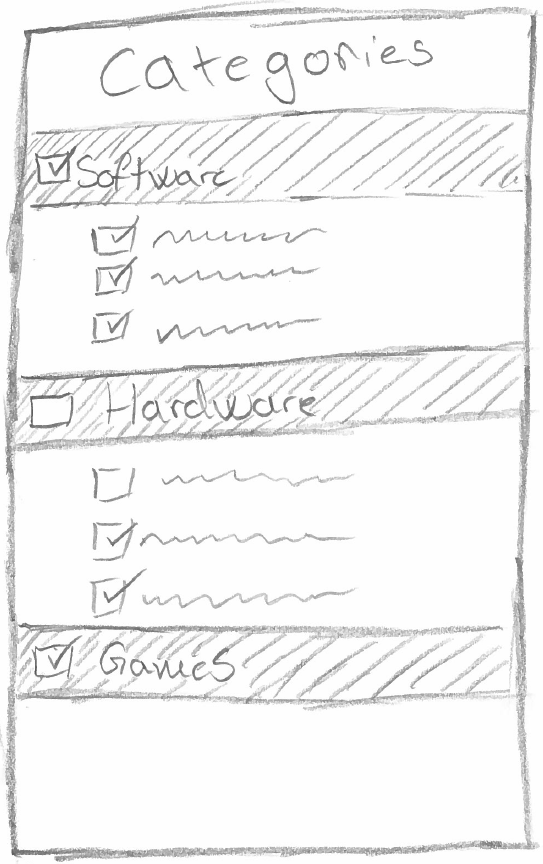
\includegraphics[width=0.7\columnwidth]{img/prototype/2.png}
\caption{Categories\label{fig:categories}}
\end{minipage}
\end{figure}

\autoref{fig:start} shows the application start screen. The user is told to scan an \ac{nfc} tag. When a tag is scanned the application checks if the user has visited the exhibition before. If the user has visited before then the exhibition information is opened, if not, then the user is asked to choose categories.

From the start screen you can also open a small menu in the bottom left corner where the user can browse for exhibitions and also pick recently visited exhibitions.

\autoref{fig:categories} is where you pick categories by clicking the check boxes. Although not present in the picture, the user should click submit in the bottom of the activity.

\begin{figure}[H]
\begin{minipage}[b]{0.5\columnwidth}
\centering

\includegraphics[width=0.7\columnwidth]{img/prototype/3.png}
\caption{Exhibition information\label{fig:exhibition}}
\end{minipage}
\hspace{0.5cm}
\begin{minipage}[b]{0.5\columnwidth}
\centering
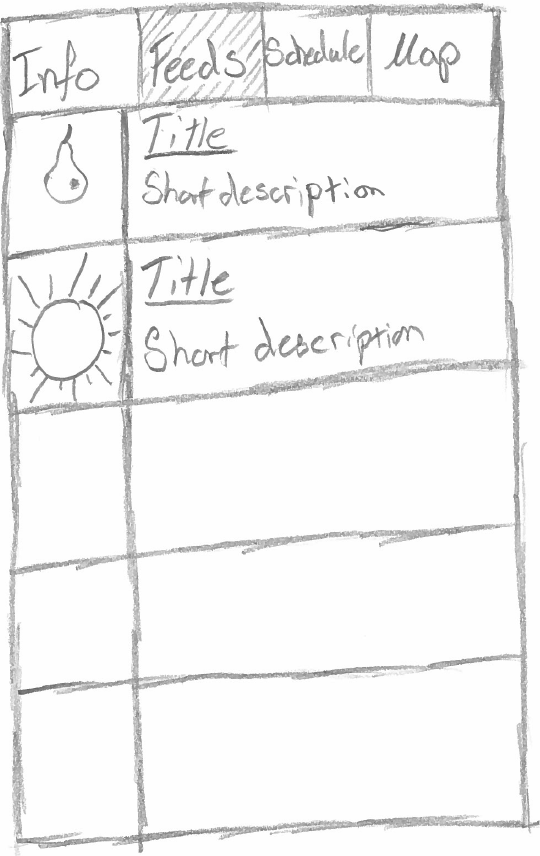
\includegraphics[width=0.7\columnwidth]{img/prototype/4.png}
\caption{Feed list\label{fig:feedlist}}
\end{minipage}
\end{figure}

When you are successfully registered at the exhibition, then you get to the core of the application. Here you can swipe between the different tabs, and also access a specific tab by clicking on it in the top menu. \autoref{fig:exhibition} shows the first tab, notice the tab bar in the top of the application showing which tab you are viewing. This is a simple welcome screen showing the exhibition icon, exhibition name, and an exhibition description.

\autoref{fig:feedlist} shows the feed list associated with the exhibition. The user receives feeds based on the chosen subscriptions that was submitted with the activity in \autoref{fig:categories}.

\begin{figure}[H]
\begin{minipage}[b]{0.5\columnwidth}
\centering
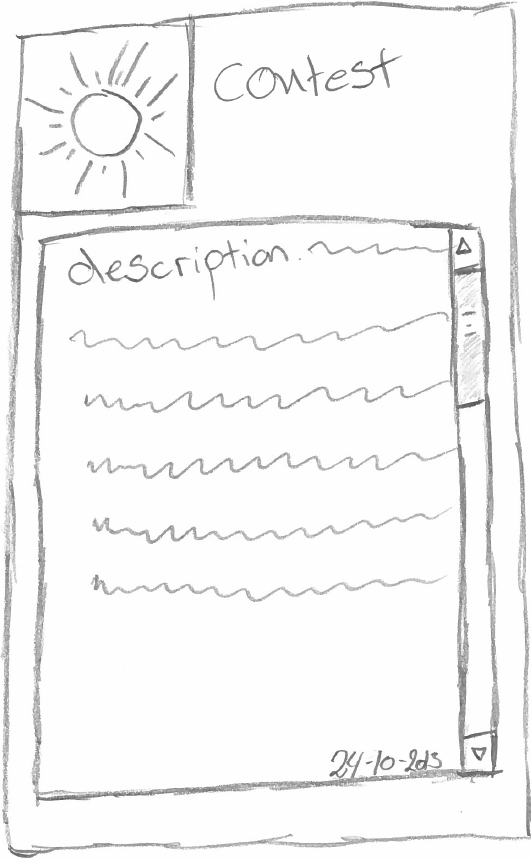
\includegraphics[width=0.7\columnwidth]{img/prototype/5.png}
\caption{Feed item\label{fig:feeditem}}
\end{minipage}
\hspace{0.5cm}
\begin{minipage}[b]{0.5\columnwidth}
\centering
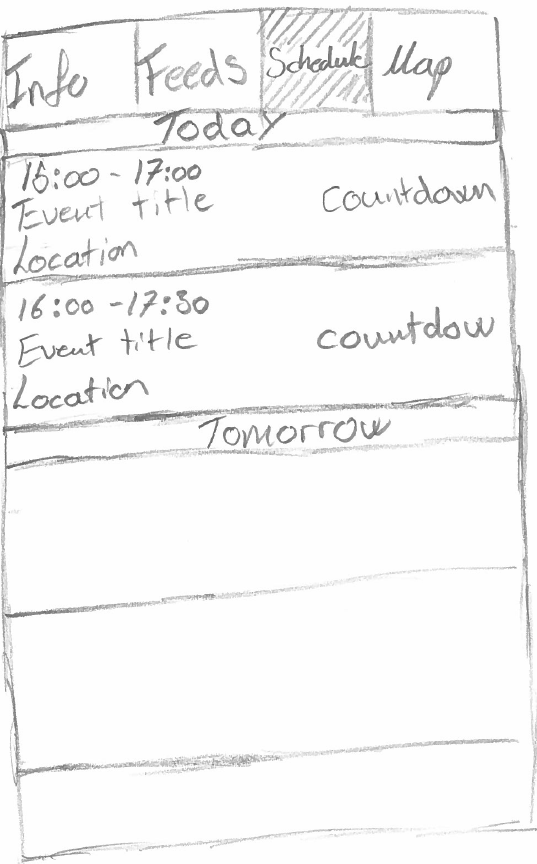
\includegraphics[width=0.7\columnwidth]{img/prototype/6.png}
\caption{Schedule\label{fig:schedule}}
\end{minipage}
\end{figure}

\autoref{fig:feeditem} is the activity shown when you click a feed item from the feed list. A feed item consists of a headline, a feed description, and it shows the icon attached to the booth which is associated with the feed item.

\autoref{fig:schedule} shows the schedule of the exhibition. The schedule items are grouped by days. Each schedule item shows the time interval of the event, a title, a location, and it shows a continuously updated countdown to the event.

\begin{figure}[H]
\begin{minipage}[b]{0.5\columnwidth}
\centering
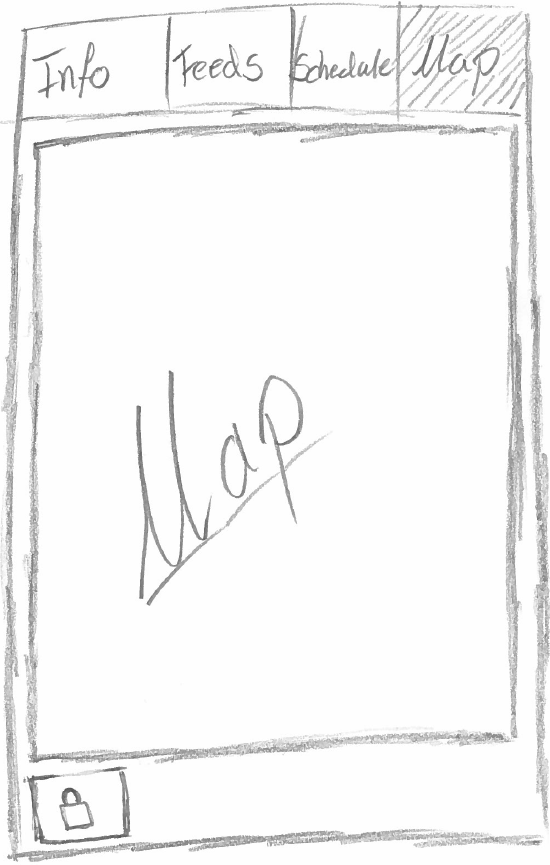
\includegraphics[width=0.7\columnwidth]{img/prototype/7.png}
\caption{Map\label{fig:map}}
\end{minipage}
\hspace{0.5cm}
\begin{minipage}[b]{0.5\columnwidth}
\centering
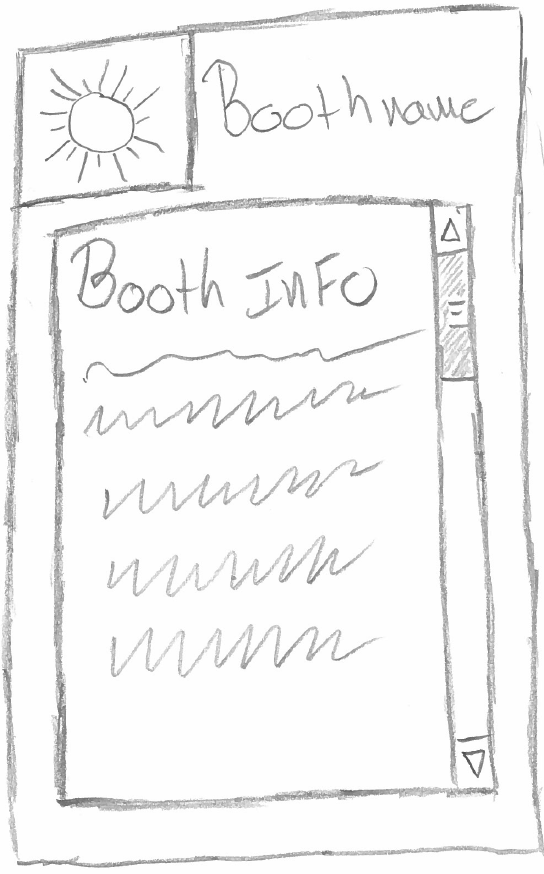
\includegraphics[width=0.7\columnwidth]{img/prototype/8.png}
\caption{Booth information\label{fig:booth}}
\end{minipage}
\end{figure}

\autoref{fig:map} shows the tab displaying the map of the exhibition. Below the map there is a lock button, which locks the user to navigating the map e.g. swiping left and right on the map. If it is not locked then swiping right will change to the schedule tab. Inside the map there should be pinned booths which can be clicked on. When clicking the booths the activity shown in \autoref{fig:booth} is opened. The booth activity shows its attached icon, a name, and information concerning the booth.

\section{Final Application Design}

The final application consists of the following activities and fragments:

\begin{description}
\item[MainActivity] This is the startup activity. This activity waits for the user to scan an \ac{nfc} tag and redirect the user appropriately.
\item[TabActivity] The core of the application, contains all the tabs i.e. fragments.
\item[ExhibitionInformationFragment] Shows information about an exhibition such as name, description, and logo.
\item[FloorplanFragment] Shows the map of the exhibition. The map contains markers for each booth which the user can click to access information about the booth.
\item[ScheduleFragment] Is a schedule for the exhibition which shows major events happening at the exhibition.
\item[FeedFragment] Is a list of news feeds based on the users subscriptions.
\item[FeedActivity] Shows the feed item when it is clicked from the feed list.
\item[CategoriesActivity] Is a list of categories, e.g. hardware, software.
\end{description}
We did not create the \textit{BoothActivity} which is showed in \autoref{fig:booth}, because we realised that we might as well show all the booth information in the marker information window on the map. This is shown later in this section.

\section*{Final design}
The following section shows our final design of our application. A run-through of each of the screen that you may encounter throughout the application.

When opening the application the first screen you encouter is one telling the user to scan an \ac{nfc} tag. The screen is shown on \autoref{fig:nfcscreen}. The windows differs from the protoype, as there is no menu in the bottom right to browse exhibitions. When the \ac{nfc} tag is scanned you are signed up to that specific exhibition and a new screen appears asking the user to choose between different categories and booths, this is to identify the users interests which will be used later by the application. This is shown on \autoref{fig:categories1}. After the user has selected their categories, they press submit. Note that after having scanned and chosen categories the first time, the next time the user opens the application and scan an \ac{nfc} tag from the same exhibition, the user does not have to choose categories and booths again.

\begin{figure}[H]
\begin{minipage}[b]{0.5\columnwidth}
\centering
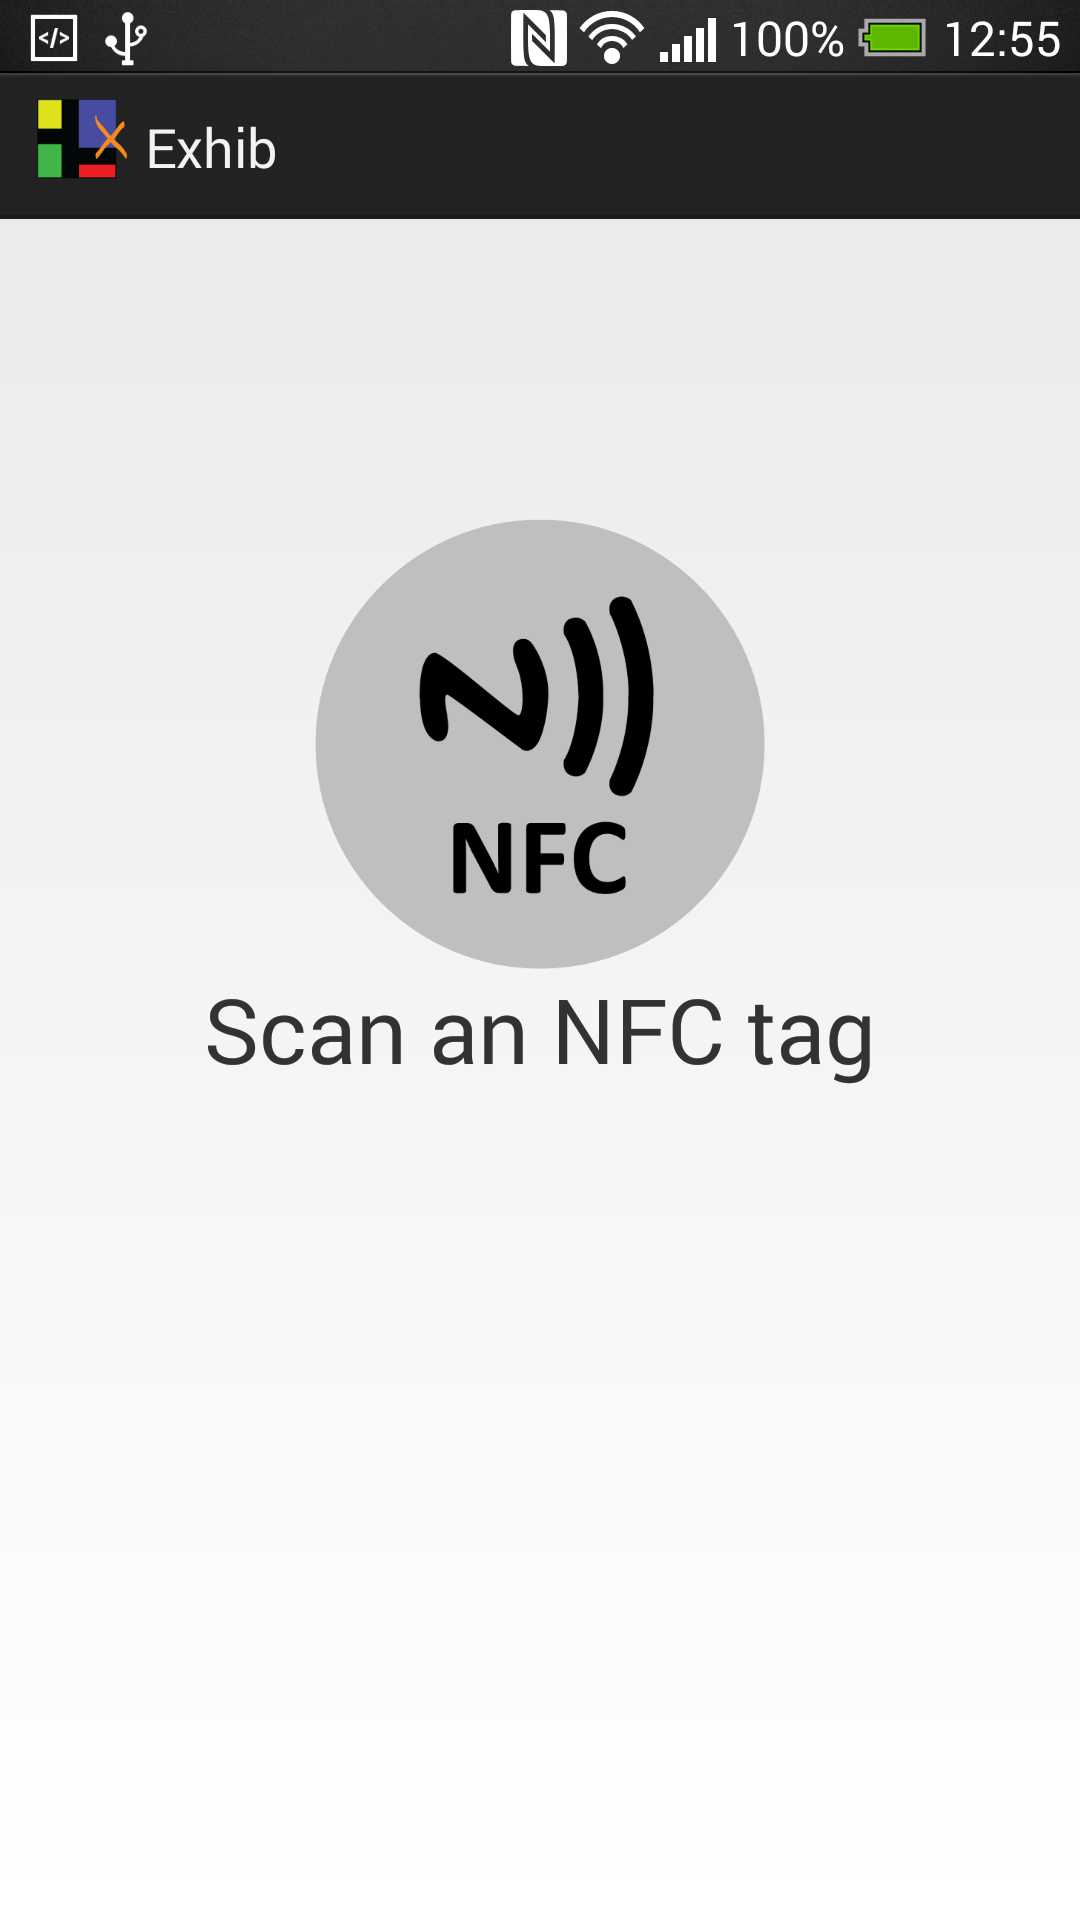
\includegraphics[width=0.7\columnwidth]{img/finaldesign/nfcscreen.png}
\caption{Start screen}
\label{fig:nfcscreen}
\end{minipage}
\hspace{0.5cm}
\begin{minipage}[b]{0.5\columnwidth}
\centering
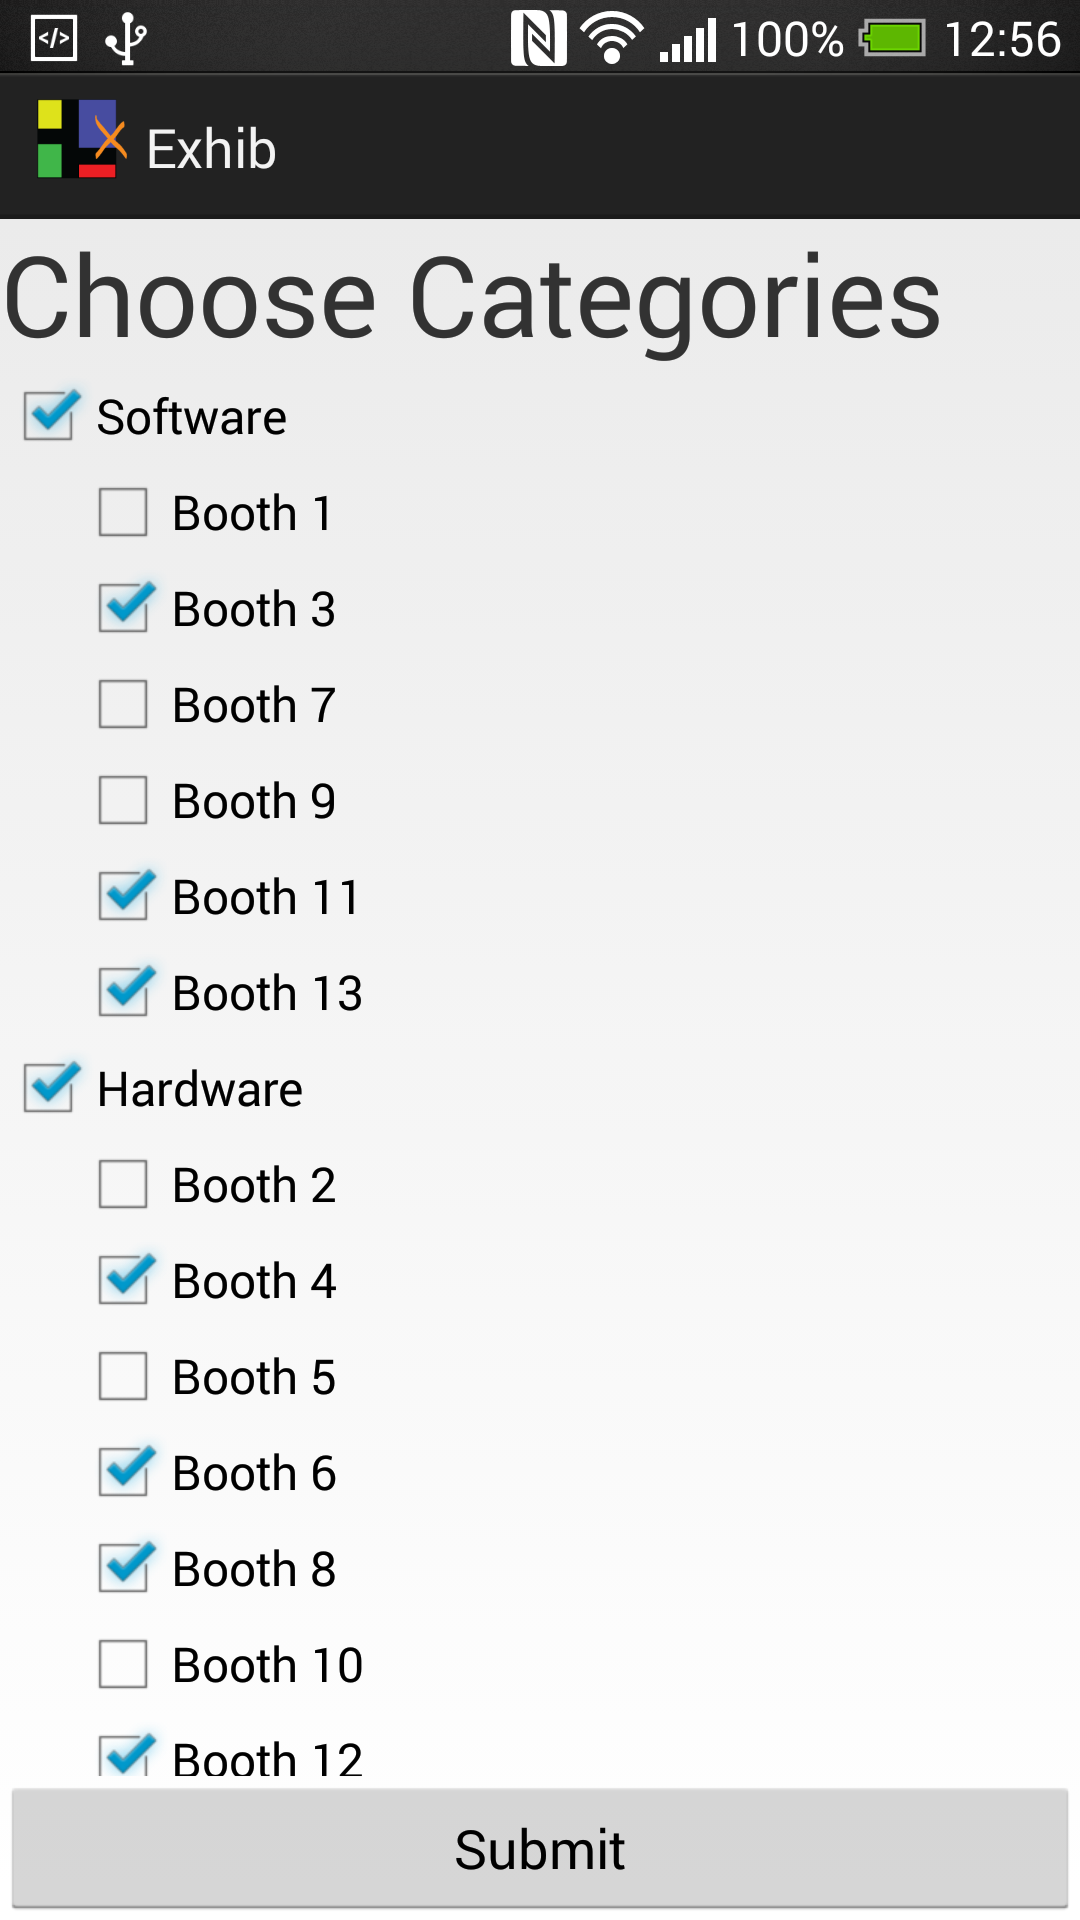
\includegraphics[width=0.7\columnwidth]{img/finaldesign/categories.png}
\caption{Categories}
\label{fig:categories1}
\end{minipage}
\end{figure}

After having submitted the categories the user want to subscribe to, the user will be taken to an "Info" tab, this is a simple tab displaying information about exhibition the user are currently at, such as exhibition logo, name and a description of the exhibition. This can be seen on \autoref{fig:infoscreen}  at the top. Next to "Info" there are three other tabs: "Feeds", "Schedule", and "Map". These four tabs can be navigated to and from, from any of the other tabs either by swiping from side to side or by clicking on the tab itself at the top.

The tab "Feeds", as seen on\autoref{fig:feedsscreen}, shows a list feeds made by booths at the exhibition. The application uses the booths that the user subscribed to before, the user only receives feeds from the booths that they subscribed to after scanning the \ac{nfc} tag. Each feed has a timestamp telling the user when it was made.

It is also possible for the user to change the booths they have subscribed to, if they want to receive different feeds. This is done by pressing the three vertical dots in the top right corner, this takes they user to the categories screen again where they can choose new categories and booths. 

\begin{figure}[H]
\begin{minipage}[b]{0.5\columnwidth}
\centering
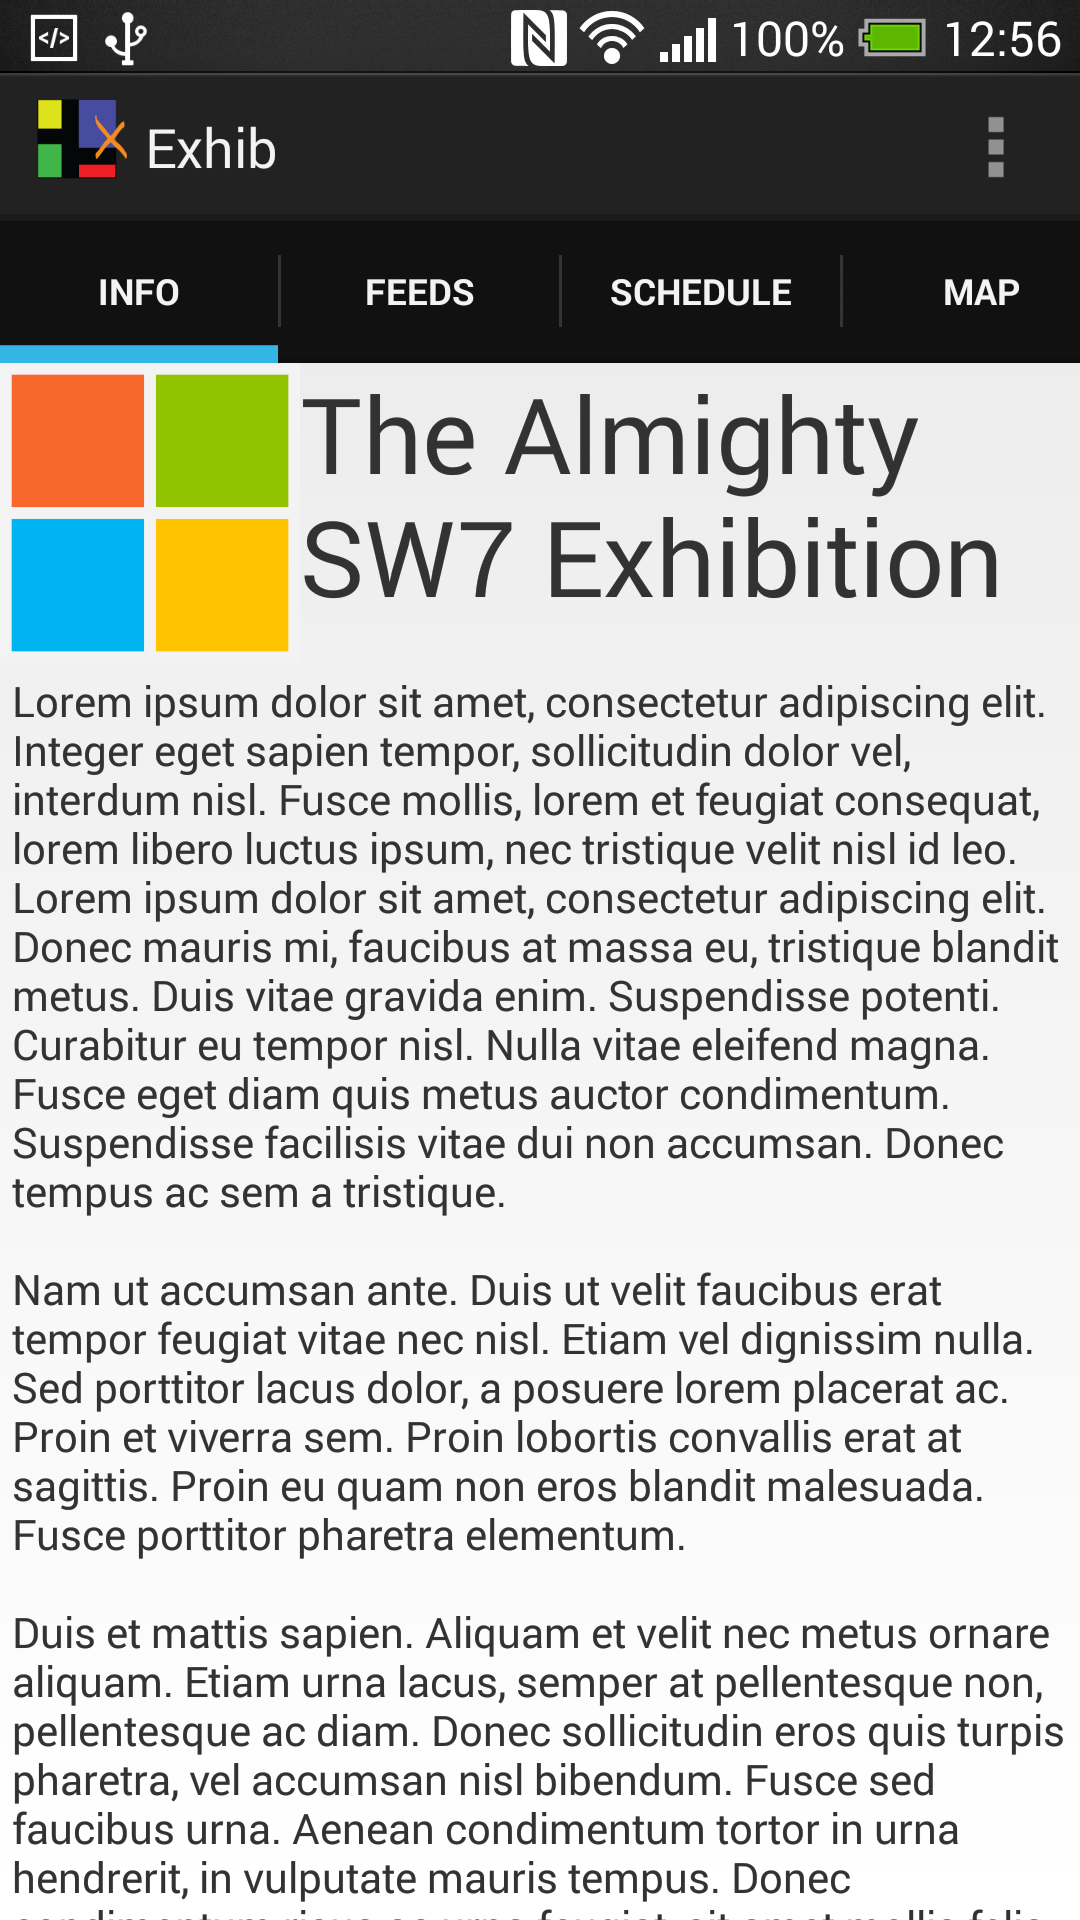
\includegraphics[width=0.7\columnwidth]{img/finaldesign/infoscreen.png}
\caption{Exhibition information}
\label{fig:infoscreen}
\end{minipage}
\hspace{0.5cm}
\begin{minipage}[b]{0.5\columnwidth}
\centering
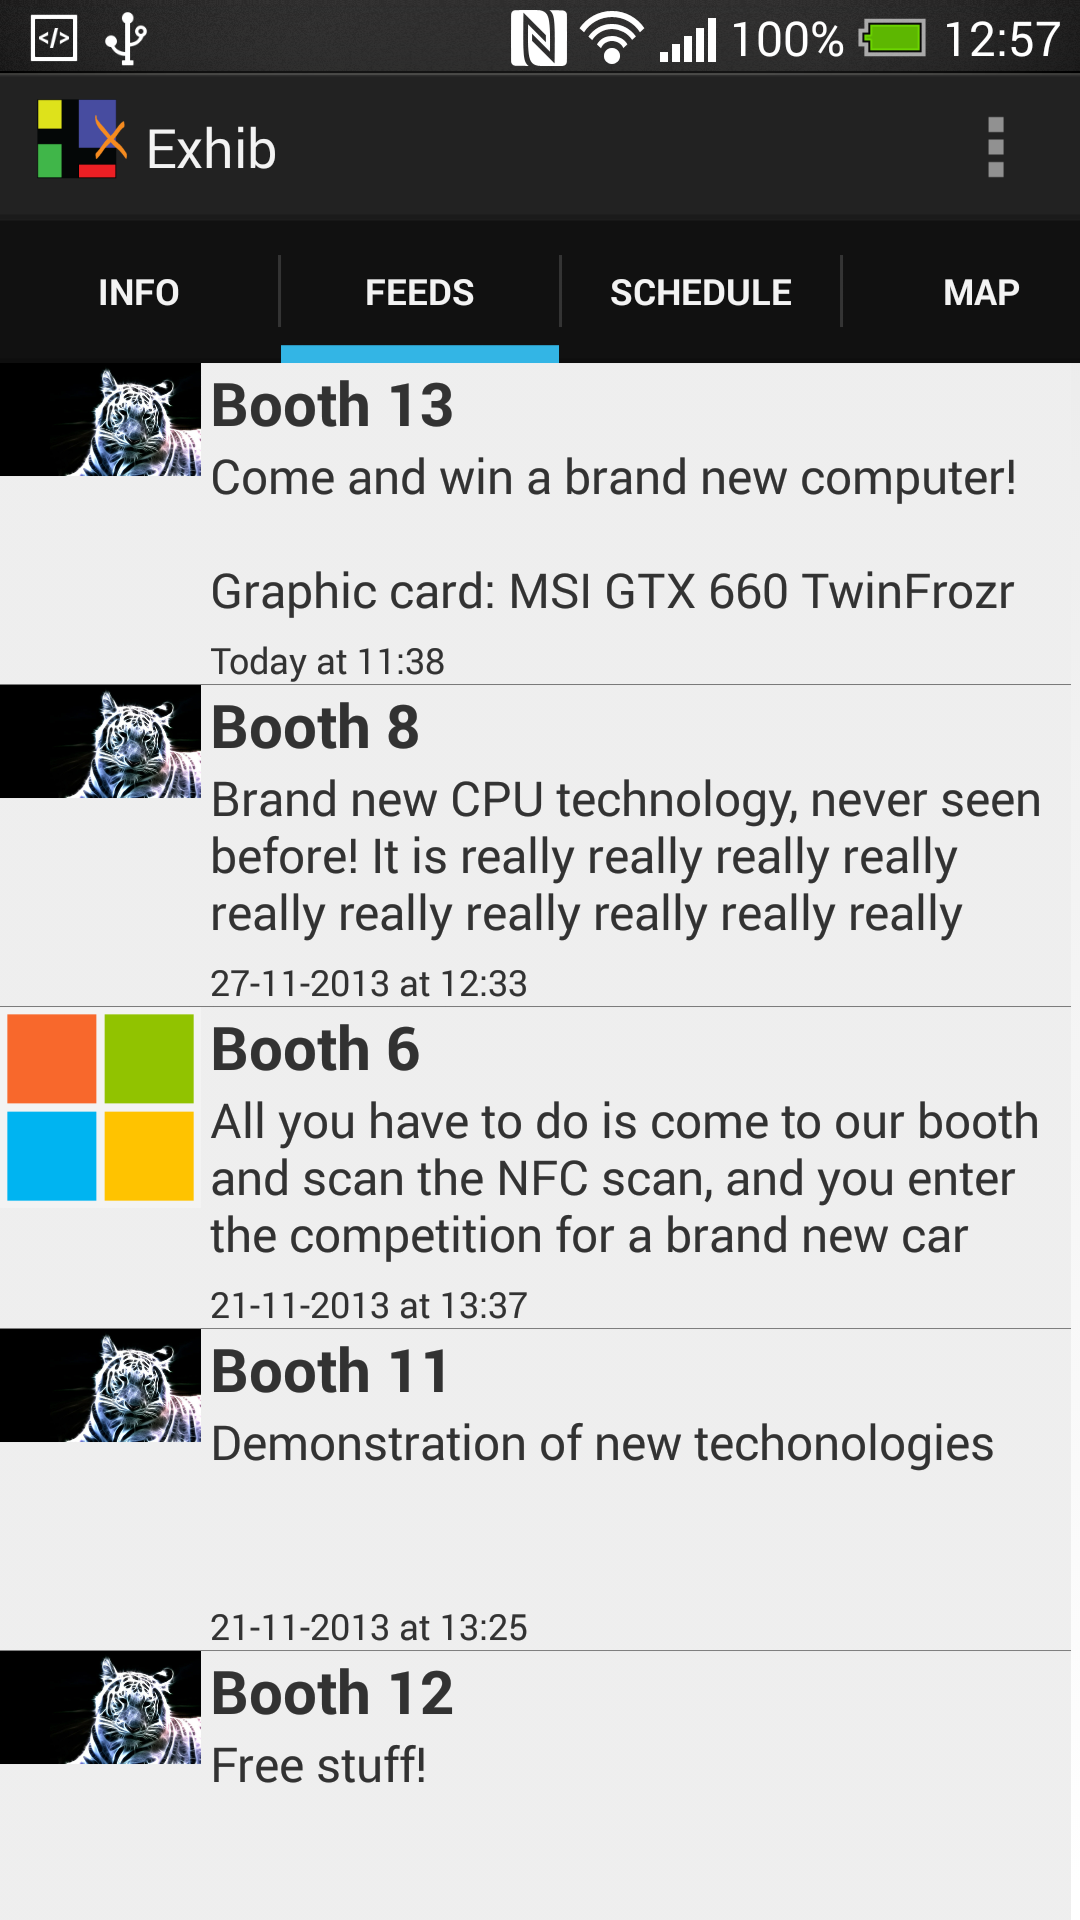
\includegraphics[width=0.7\columnwidth]{img/finaldesign/feedsscreen.png}
\caption{Feed list} 
\label{fig:feedsscreen}
\end{minipage}
\end{figure}

Some of the feeds are too long to display all the text in the list of feeds, so in order to read the full feed you can press the feed and a pop-up will come up displaying the full feed, as shown on \autoref{fig:popupfeed}. This is different from the prototype, because we thought it would be more convenient for the user to have a pop-up. During the exhibition, the booths might send new feeds, when this happens a button will be displayed, telling the user that more feeds are available, allowing them to choose when they want to load the new feeds so they always can make sure they have read all feeds before loading new ones. This can be seen on \autoref{fig:feedsnewitem}.

\begin{figure}[H]
\begin{minipage}[b]{0.5\columnwidth}
\centering
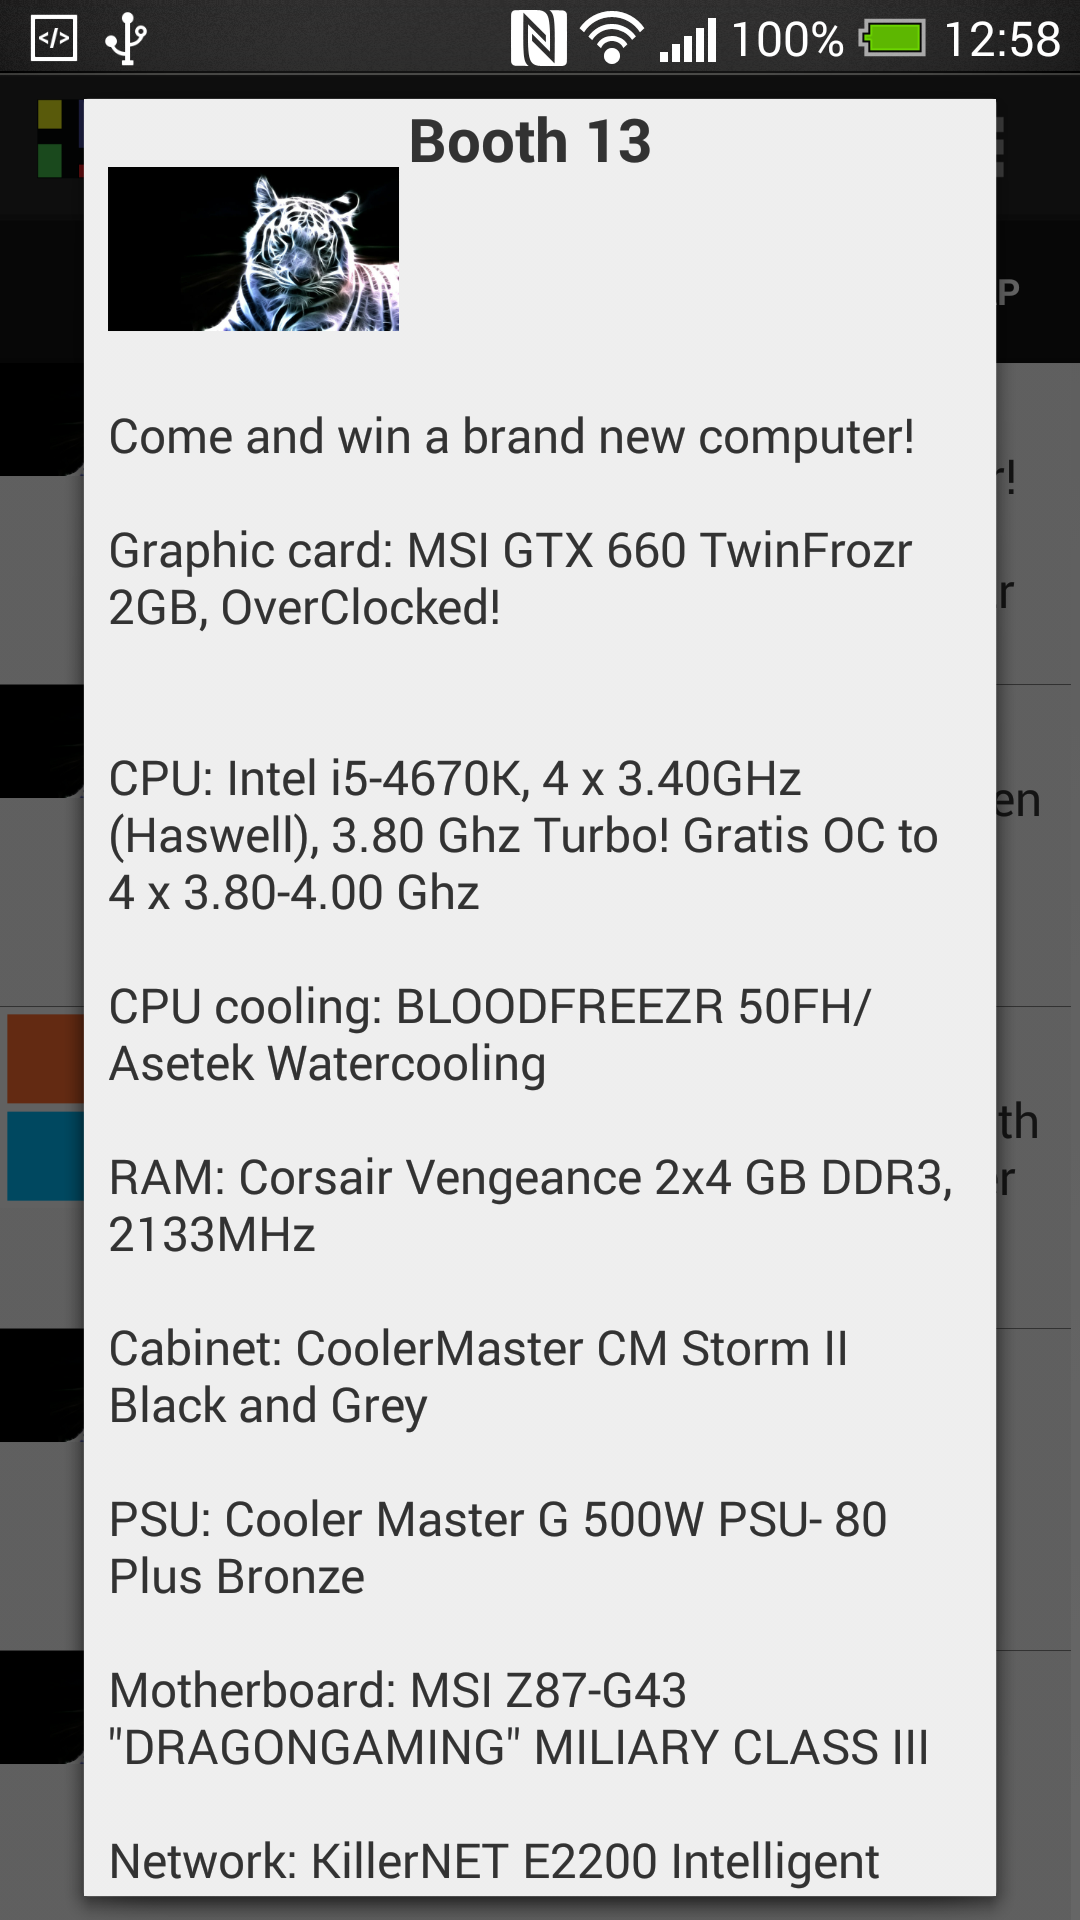
\includegraphics[width=0.7\columnwidth]{img/finaldesign/feedspopup.png}
\caption{Feed popup}
\label{fig:popupfeed}
\end{minipage}
\hspace{0.5cm}
\begin{minipage}[b]{0.5\columnwidth}
\centering
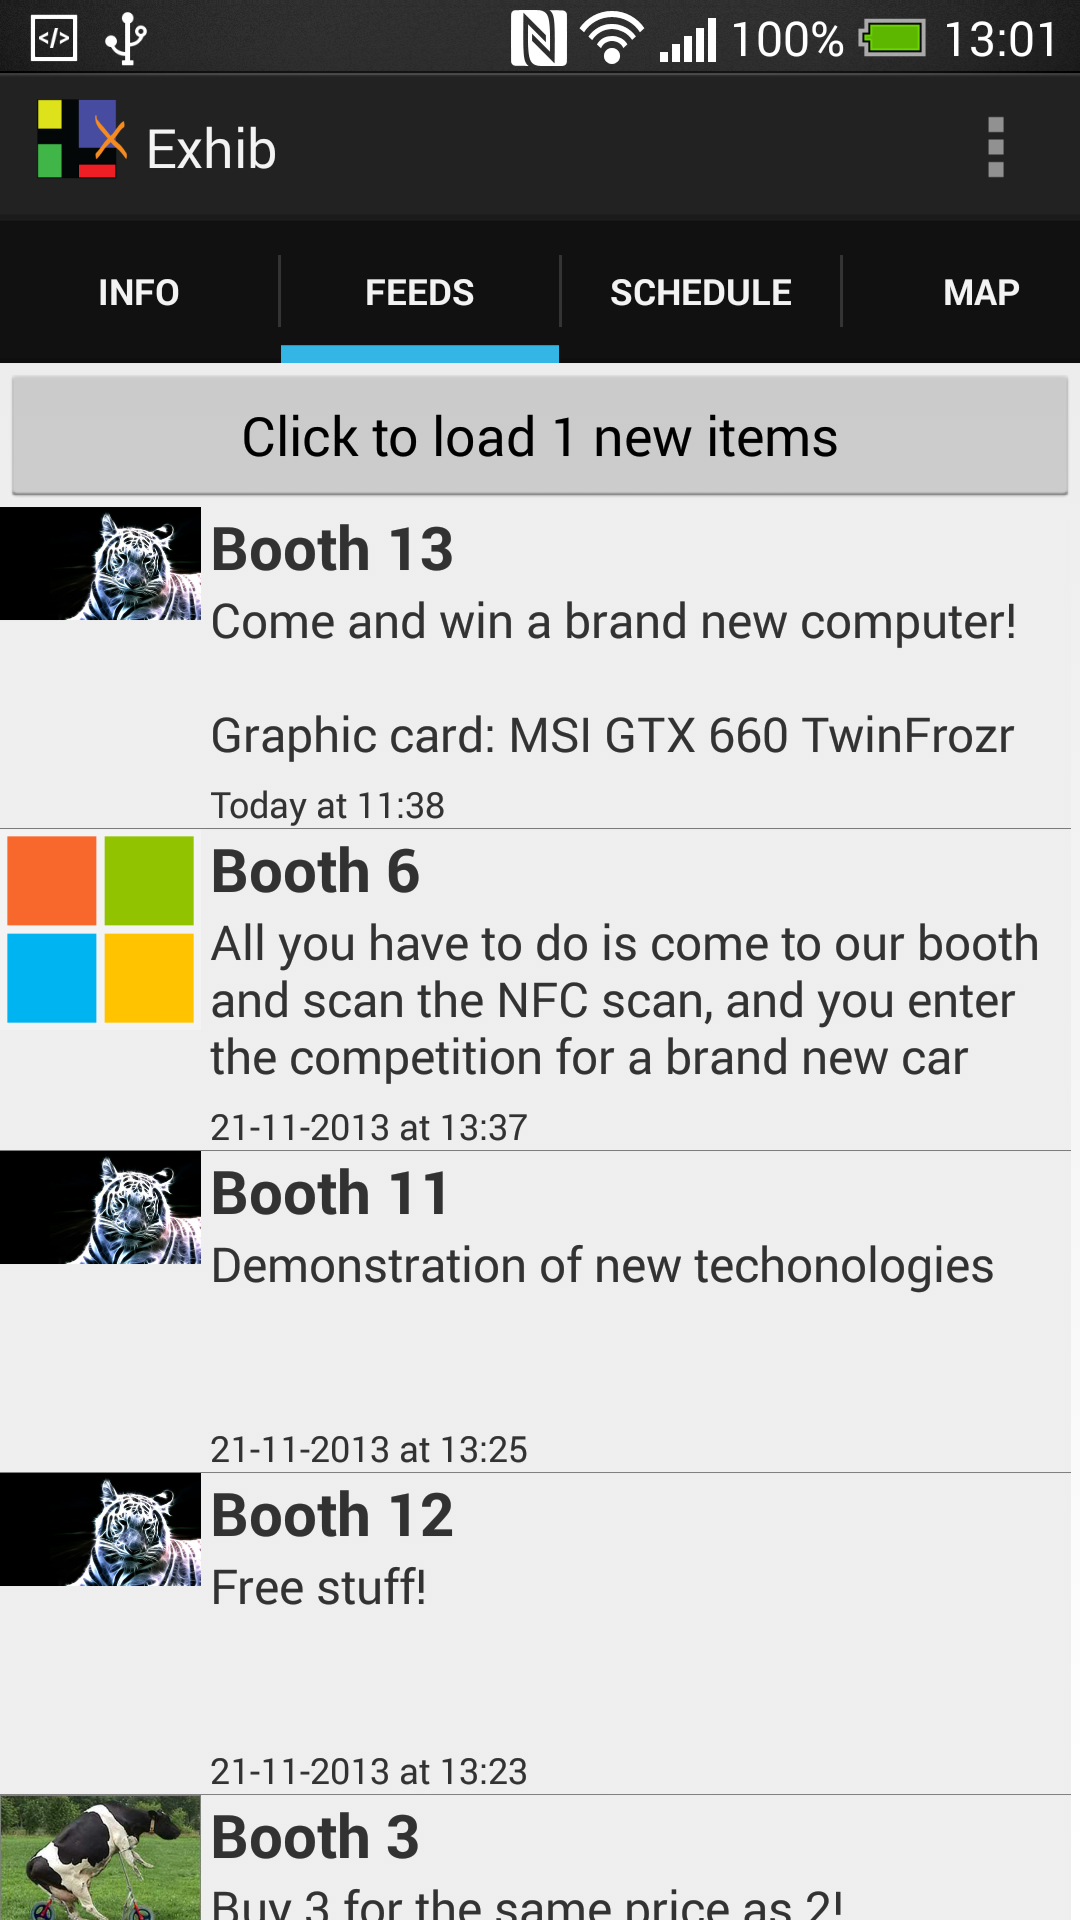
\includegraphics[width=0.7\columnwidth]{img/finaldesign/feedsnewitem.png}
\caption{New feed item}
\label{fig:feedsnewitem}
\end{minipage}
\end{figure}

The "Schedule" tab shows the events that is going on at the exhibition itself, could be a company presenting some new hardware or software at the main stage. This can be seen on \autoref{fig:schedule1}. Each event in the schedule has a countdown to when it will happen. 

The last tab is the map, this is a map over the exhibition, displaying all the booths on the exhibition. If you scan an \ac{nfc} on a booth the map will snap to that booth on the map and display a red circle to show where you are, this can be seen on \autoref{fig:map1}. You can also press the info icon on each booth, to receive information about this booth.

\begin{figure}[H]
\begin{minipage}[b]{0.5\columnwidth}
\centering
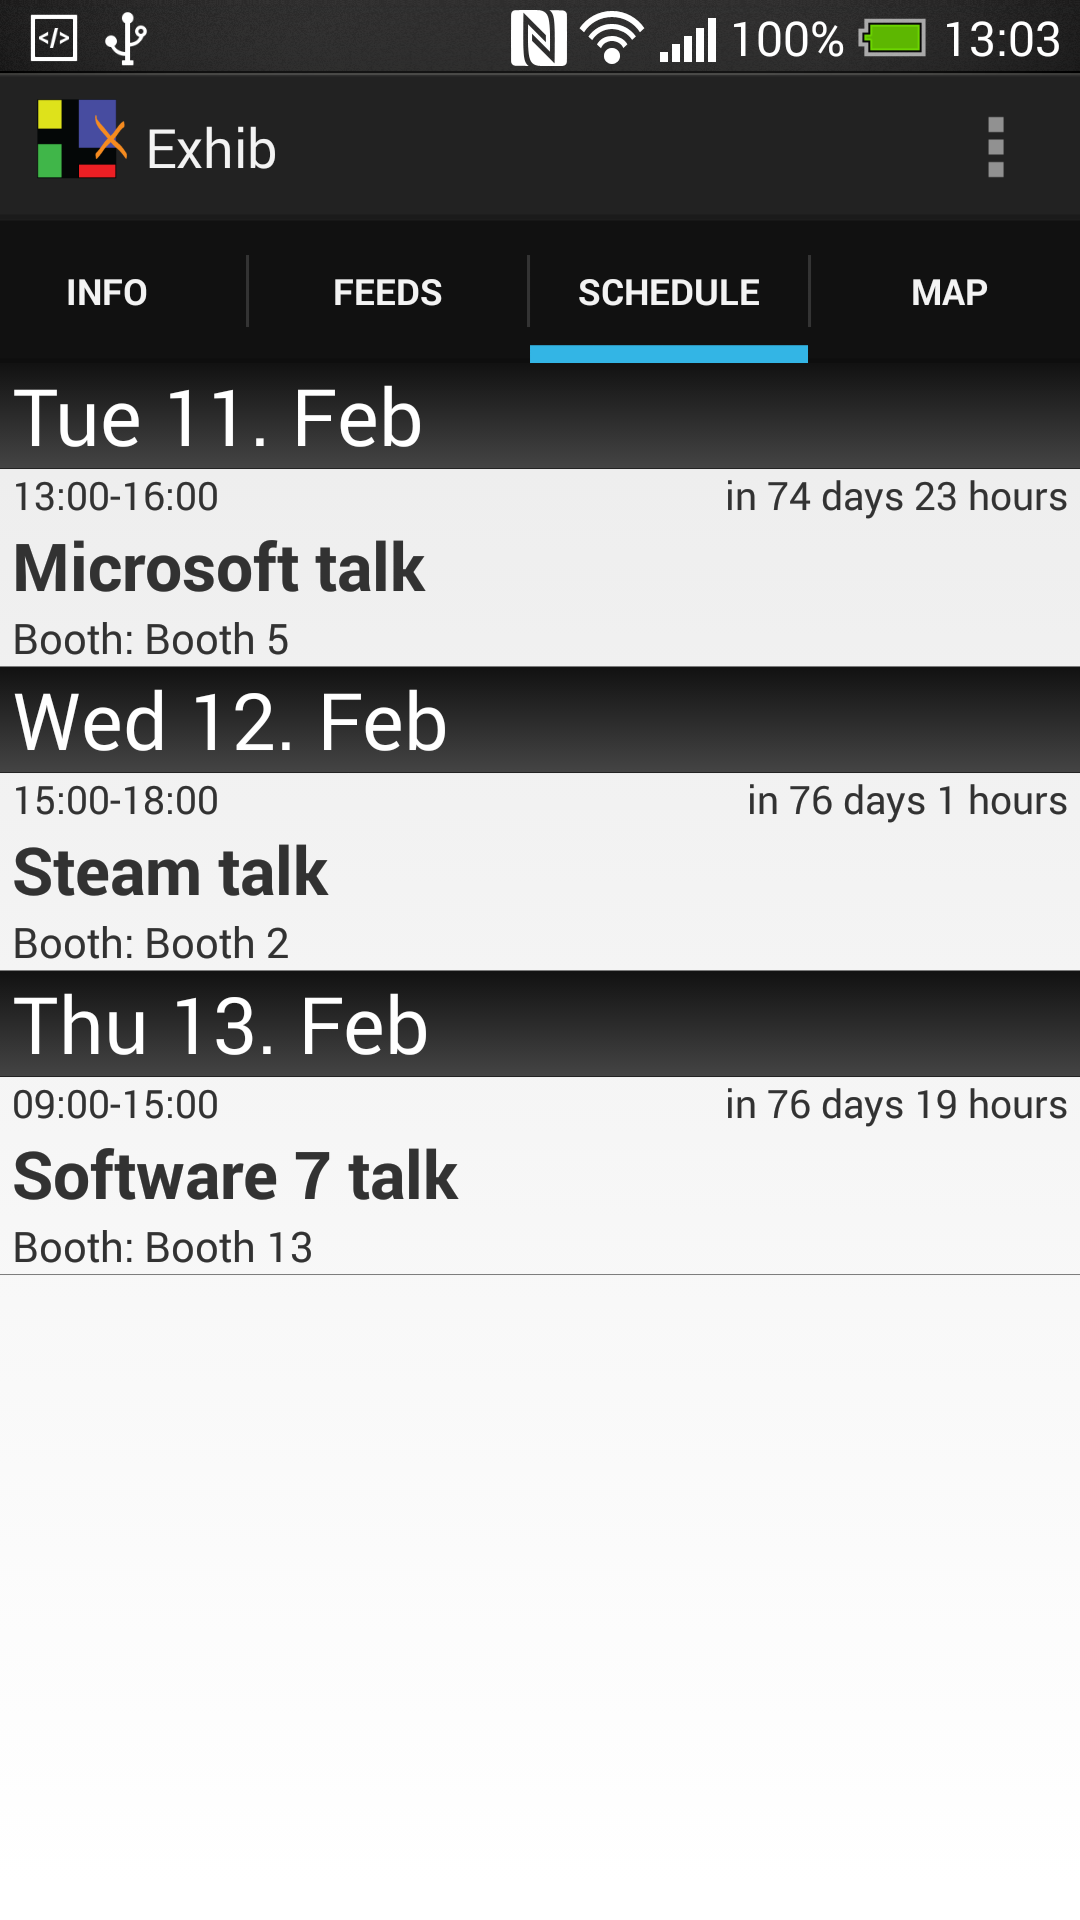
\includegraphics[width=0.7\columnwidth]{img/finaldesign/schedule.png}
\caption{Schedule}
\label{fig:schedule1}
\end{minipage}
\hspace{0.5cm}
\begin{minipage}[b]{0.5\columnwidth}
\centering
%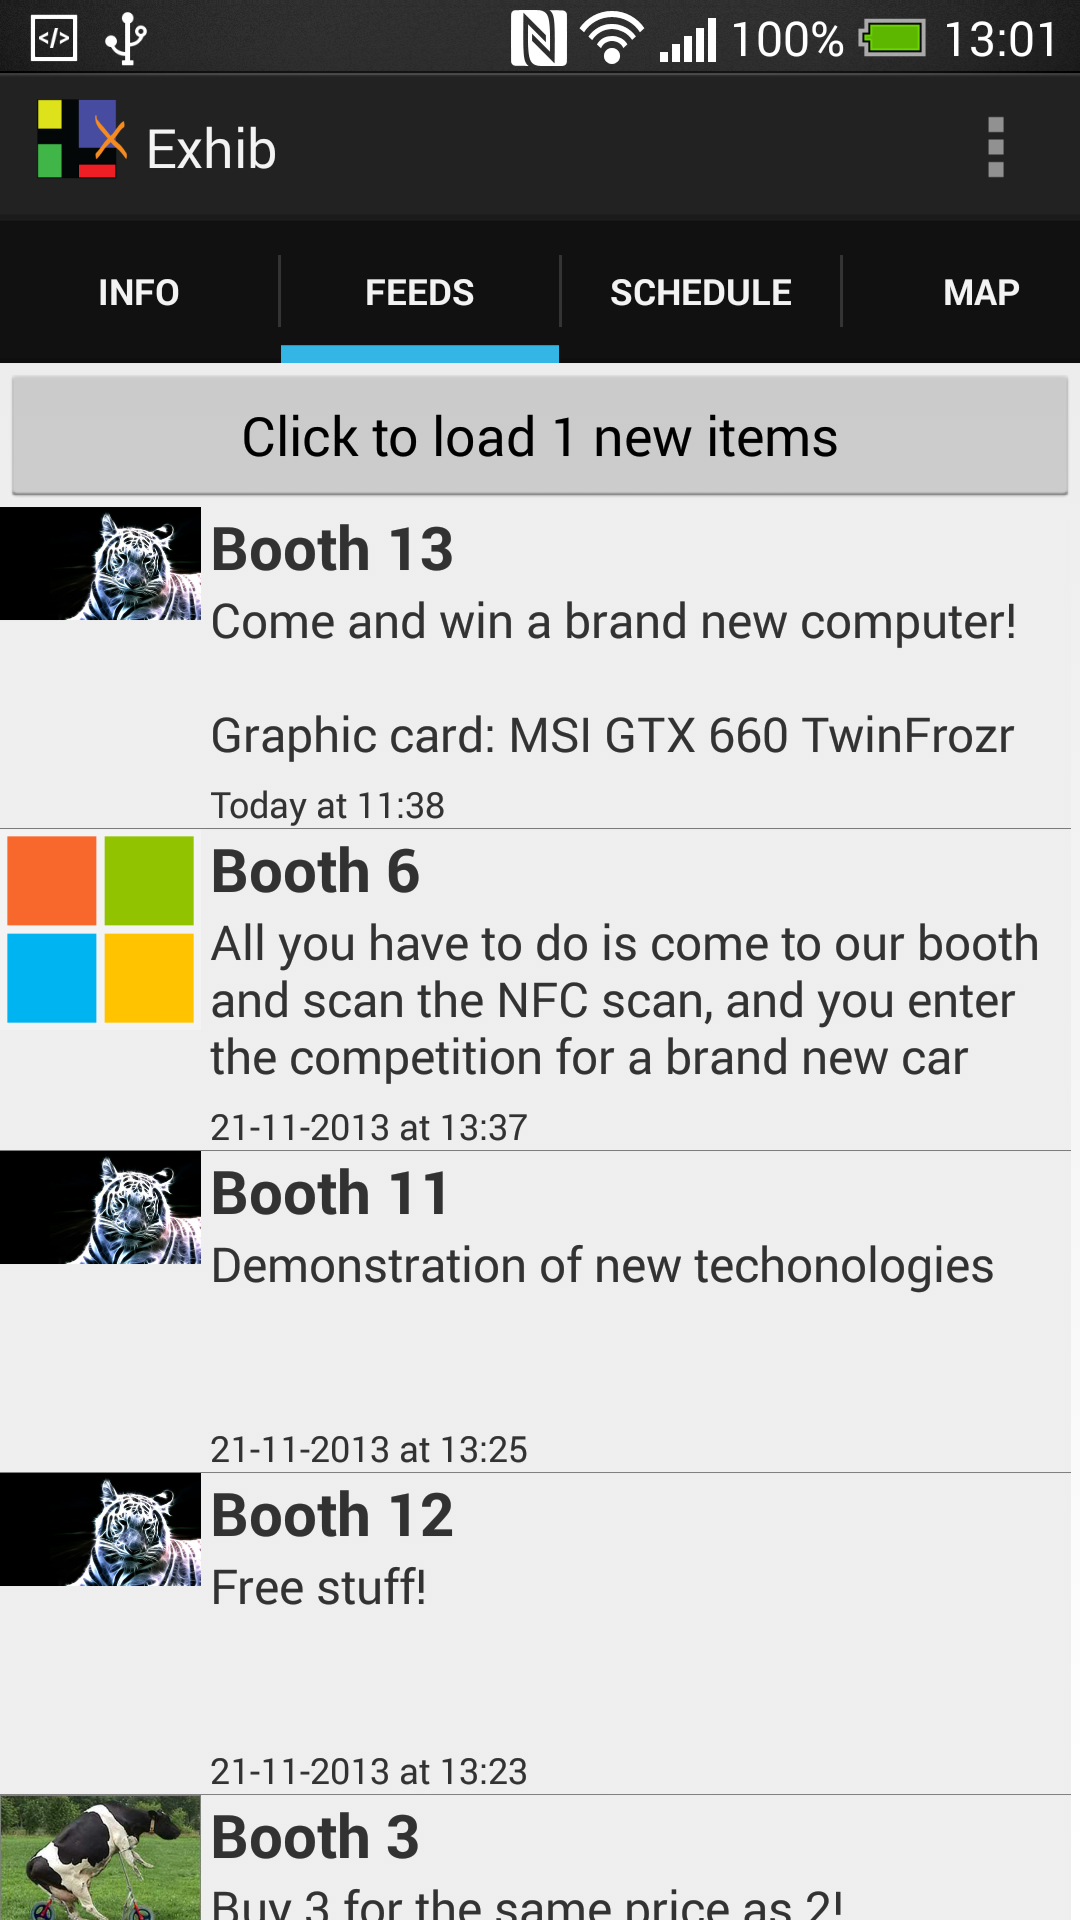
\includegraphics[width=0.7\columnwidth]{img/finaldesign/feedsnewitem.png}
\caption{Map}
\label{fig:map1}
%
\missingfigure{}
\end{minipage}
\end{figure}\todo{Picture of map goes here}

\autoref{fig:flowchart} show the application flow between these different activities. Note that the \textit{TabActivity} consists only of tabs, each tab is defined in a fragment.

\begin{figure}[H]
\centering
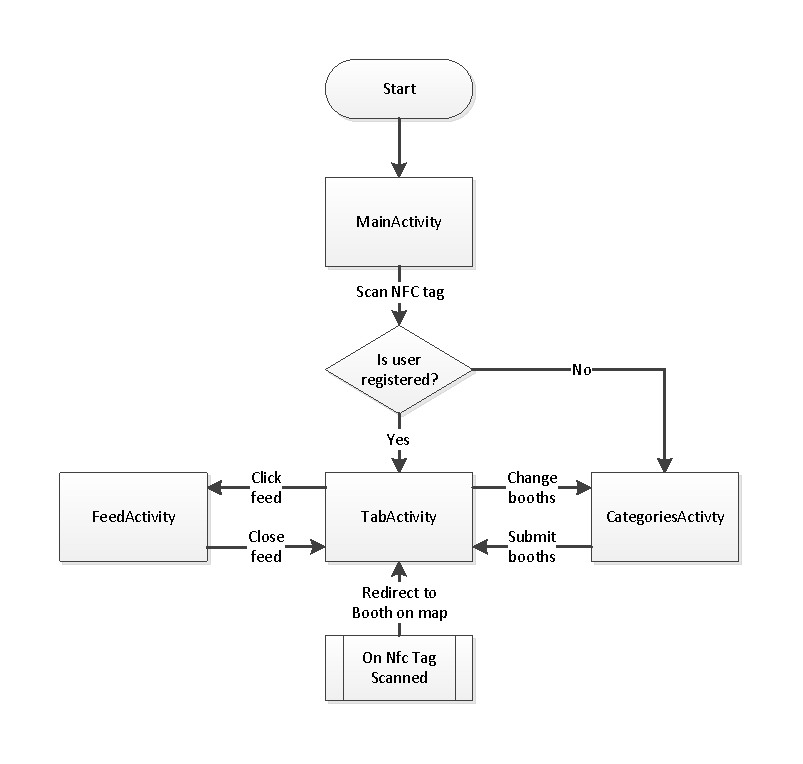
\includegraphics[width=\columnwidth]{img/appFlowchart.pdf}
\caption{Application actvity flow\label{fig:flowchart}}
\end{figure}
\todo{Pictures and description of the finished application}


\chapter{Back-end design}
This chapter describes the communication between server and client, aswell as the design choices and
implementation of database. \todo{Bør database være et kapitel for sig selv?}

\section{Communication}
\label{sec:com}

The communication betweeen the client application and the server is done by HTTP POST requests.
The client sends a HTTP POST request to the server containing a certain list of parameters which
define what the server is supposed to do. All requests must take atleast two required parameters, a \textit{RequestCode} and a
\textit{Type}.

\textit{RequestCode} is an integer that is simply passed through the server, it is not handled in any
way on the server. The purpose of the RequestCode parameter is to distinguish the request on the client allowing
it to execute the appropriate function.

\textit{Type} is used to identify the request. A typical request is to get a list of feeds, and the
value of the \textit{Type} parameter would be ``GetFeeds'' in this case.\\

Depending on the \textit{Type} of the request, additional parameters may be required.\\

As an example, \textit{GetFeeds} takes the following parameters:
\begin{itemize}
\item RequestCode
\item UserId
\item Limit
\end{itemize}

The approach is to process the request on the serverside, and make the right calls to the
database. The server will then return a JSON object containing all the relevant information that was
requested. This JSON object can easily be parsed on the client side. The reason why we chose JSON as
a format is because it is well supported and easy to generate in both android and PHP.

\begin{lstlisting}[language=phpstyle, caption=getFeeds function call]
$requestCode = $_POST["RequestCode"];

switch ($_POST['Type']) {
        case "GetFeeds":
            getFeeds($con, $_POST['UserId'], $_POST['Limit']);
            break;
}
\end{lstlisting}

\begin{description}
\item \textbf{Line 1: }Get the \textit{RequestCode} parameter.
\item \textbf{Lines 3-7: }If \textit{Type} equals ``GetFeeds'', call the getFeeds function.
\end{description}

\todo{Nævn de andre cases, måske her?}

\begin{lstlisting}[language=phpstyle, label=lst:getFeeds, caption=getFeeds function]
function getFeeds($con, $userId, $limit) {

    global $requestCode;

    #Escape special characters to avoid SQL injection attacks
    $userId    = $con->real_escape_string($userId);
    $limit     = $con->real_escape_string($limit);

    $query =   "SELECT feeds.id, feeds.boothid, feeds.header, feeds.description, feeds.feedtime, userbooths.userid, companies.logo, booths.name ".
        "FROM feeds ".
        "LEFT JOIN userbooths ".
        "ON feeds.boothid = userbooths.boothid ".
        "LEFT JOIN booths ".
        "ON feeds.boothid = booths.id ".
        "LEFT JOIN companies ".
        "ON booths.companyid = companies.id ".
        "WHERE userid = ".$userId." ".
        "AND sub = 1 ".
        "ORDER BY feeds.feedtime DESC ".
        "LIMIT "$limit;

    $result = $con->query($query);

    $json = array();
    while($row = $result->fetch_object()) {
      array_push($json, $row);
    }
    echo $requestCode;
    echo json_encode($json);
}
\end{lstlisting}%$

\begin{description}
\item[Line 1] The function takes three parameters, the MySQLi object which has a connection
  established to the database, the user id from the client, and the limit which is also given by the client.
\item[Line 3] Since the \textit{RequestCode} is always a required parameter the variable is global.
\item[Lines 6-7] Escape special characters to avoid malicious SQL injections.
\item[Lines 9-20] Create the SQL query with the user id and the limit paramter.
\item[Line 22] Execute the query.
\item[Lines 24-29] Get the results from the database and push them to the JSON array. When
  all of the results have been pushed to the array, the \textit{RequestCode} will be echoed and then
  a JSON encoded version of the array.
\end{description}

As seen on line 29 in \autoref{lst:getFeeds} the result is JSON encoded and then echoed. An example of a result from the \textit{GetFeeds} type request could look like the following:

\begin{lstlisting}[language=json, label=lst:jsonResult, caption=Example result from a request with type: \textit{GetFeeds}]
1[
    {
        "id": "18",
        "boothid": "2",
        "header": "asdf",
        "description": "Super.",
        "feedtime": "2013-10-02 12:41:02",
        "userid": "1",
        "logo": "microsoftlogo.png",
        "name": "Microsoft XBOX"
    },
    {
        "id": "17",
        "boothid": "2",
        "header": "short header",
        "description": "short description.",
        "feedtime": "2013-10-02 11:43:28",
        "userid": "1",
        "logo": "microsoftlogo.png",
        "name": "Microsoft XBOX"
    }
]
\end{lstlisting}

Note the number before the array in \autoref{lst:jsonResult}, this is the request code.

All of the requests to the server follows this principle. A request is made, the query is run and data is gathered, and lastly the result is returned as a JSON object that the client reads.\\\\
Our types of requests are as follows:
\begin{itemize}
\item \textbf{GetFeeds}\\
 Will return all the necessary data about a certain number of feeds. They are sorted to return the newest feed first and then the next number of feeds that coresponds to the given limit parameter.
\item \textbf{CreateUser}\\
  Creates a new user in the database and returns the userid.
\item \textbf{GetNewFeeds}\\
  Returns data about all new feeds since the last update. This means that the user can manually fetch all new feeds.
\item \textbf{CheckFeeds}\\
  Check if any new feeds are available, and if such the number of new feeds will be returned.
\item \textbf{GetOldFeeds}\\
  Load a certain number of feeds that are older than the current oldest feed showing. This allows the user to load the next batch of feeds.
\item \textbf{GetSchedule}\\
  Returns relevant data about the schedule of the exhibition. Used for the schedule tab on the android application.
\item \textbf{GetExhibitionInfo}\\
  Returns all information about the exhibition, such as the description and logo.
\item \textbf{GetCategories}\\
  Returns a list of categories, and the booths of this category, that are associated with the current exhibition. It also contains a flag that shows whether the user is currently subscribed to a booth or not.
\item \textbf{SetCategories}\\
  This request is run when the ``submit'' button is pressed in the category chooser. This updates the booths that the user is subscribed to in the databse.
\end{itemize}

\section{Database}
We are using a MySQL database with the MyISAM storage engine and which is located at a remote server. \todo{info om hvor osv.?}

The server is to contain all data about each exhibition, the companies at the exhibition, the feeds, the schedule, and some basic information about the users.

\begin{figure}[H]
\centering
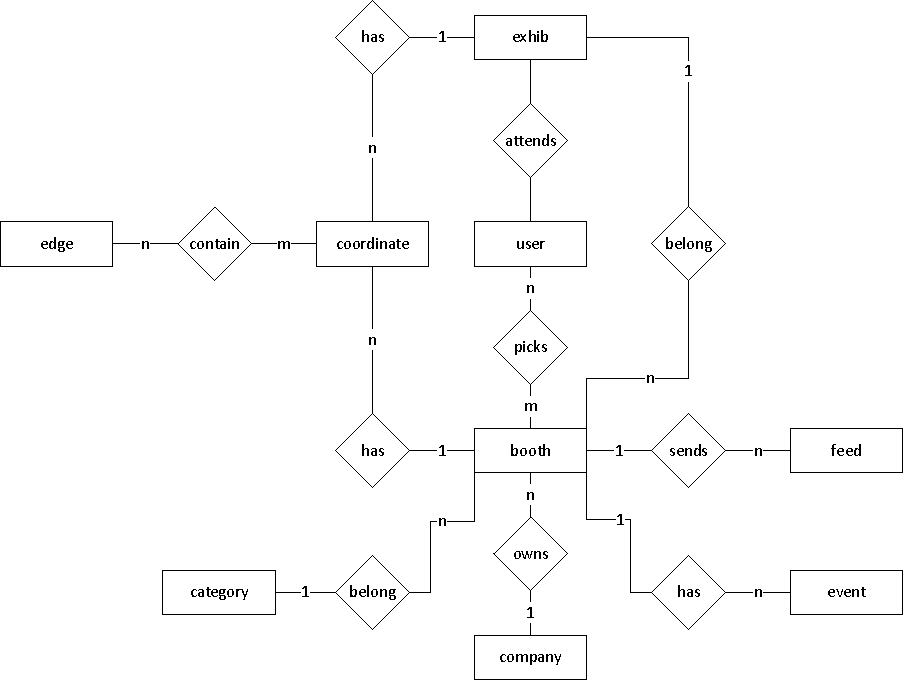
\includegraphics[page=1,width=1\linewidth]{img/sw7ERD.pdf}
\caption{Entity-relation diagram}
\label{fig:erd}
\end{figure}
\todo{ERD skal opdateres!!}

%%% Local Variables: 
%%% mode: latex
%%% TeX-master: "../master"
%%% End: 


\bookmarksetup{startatroot}% dette skulle stoppe part, så conclusion får indryk. Problemet i skrivende øjeblik er at chapters har samme indryk uafhængigt af parts
\addtocontents{toc}{\bigskip}%laver ekstra mellemrum

\chapter{Conclusion}
The focus of this project was to make an application that would improve the experience involving both organisers and attendees at an exhibition.
This is defined in our problem definition in \chapref{chap:intro}:
\begin{quote}
\textit{"How can we ease the creation of exhibitions, while enhancing the user's experience by providing them with relevant information while at the exhibition."}
\end{quote}
In order to give each user a customisable experience, the first problem that had to be solved was how the users should be identified at an exhibition. We chose to do this using \ac{nfc} tags because they allow us to register when a user scans them and thereby providing them with a unique user ID.
 
With the identification technology in place we started focusing on the rest of the system. The system itself is split into three parts, a website, a server and a mobile application.

The website is a tool for the exhibition organisers, with the purpose of creating and editing exhibitions. They are able to set up an exhibition and its floor plan. This allows them to plot in the location of booths and the walk paths around the exhibition. Each booth has a company and a categories assigned to them, which is used on the mobile application to allow the user to specify what type of booths they are interested in. The organisers can also create feeds that are related to a specific booth and create events for a global schedule that is related to the entire exhibition. We managed to implement all the features for the website mentioned in \secref{sec:exhibsystem}. However, the creation of feeds is only implemented with limited functionality. Each booth should be able to create their own feeds and schedule entries, however this would require a login system which we decided not to focus on for this project. The organisers and the booth organisers can still create feeds through the website for a specific booth, but there is no control of who creates feeds for which booth. The organisers are also able to load an old exhibition and edit it.

The mobile application is implemented on the Android platform. The first time a user scans an \ac{nfc} tag they are asked to select which booths they want to subscribe to. Each booth belong to different categories, assigned by the exhibition organiser. After the user has signed up for an exhibition they are taken to the tab activity where they can navigate between four tabs; ``Info'', ``Feeds'', ``Schedule'', and ``Floor plan''.

The ``Info'' tab provides the user with information about the exhibition, such as the name and a description. The ``Feeds'' tab shows the user feeds from the different booth they have subscribed to, the user can, if wanted, change their subscriptions, allowing them to fully customise which booths they want to receive feeds from. The user can also click a feed and get a pop up with the full description of that feed. The ``Schedule'' tab shows a list of different events happening at the exhibition. The user will only receive events from the booths they are subscribed to. Each schedule entry also has a time counter showing how long until the event. The ``Floor plan'' shows the floor plan that the organisers created with the tool, it also shows all the booths and walk paths around the exhibition. If a user scans a tag on a booth with the application closed, the application will open on the ``Floor plan'' tab and snap to the booth. A red dot is shown on the floor plan to indicate where the booth is placed. They are also able to click another booth on the floor plan and navigate to it by clicking the button. We managed to implement all features for the mobile application mentioned in \secref{sec:exhibsystem} except for one. The user is not able to browse for exhibitions or browse recently added exhibitions.

If the user arrives at a new exhibition and scan another \ac{nfc} tag, they will sign out of the previous exhibition and sign up for the new exhibition and be prompted to choose new booths. 

Based on the tests performed in \chapref{chap:tests} we can guarantee that the mobile application is working as intended. We have not made any graphical user interface tests, to ensure the design of our mobile application and website. We have managed to create a system for helping organisers create exhibitions while also enhancing the user experience for attendees at an exhibition, which was the of the project.\label{chap:conclusion}

\chapter{Future Work}
\begin{description}
%\item[Other map items] We only show booths and paths on the map. It is not possible to show a stage or a 'you are here' stand. There is a workaround for this at the moment, you can create a booth instead, but it might confuse the exhibition organisers.
\item[Exhibition schedule] The exhibition organisers can not create a schedule bound to the exhibition, you can only create a schedule for a booth.% This is also part of the lack of functionality mentioned above.
\item[Exhibition statistics] Right now we save how many times each user has visited a booth, i.e. each time they scan an \ac{nfc} tag at a booth. All the statistics should be shown to the exhibition organisers.

Metrics could be: How many subscribers each booth has, how many times navigation to a booth has been requested, and how many users an exhibition has.
\item[User recommendations] Based on the users subscriptions and which booths the user has visited, we could recommend other booths which belongs to the same category.
\item[Tag scanned event] When an \ac{nfc} tag is scanned we could provide the user with different actions, such as: Navigate from this booth to another, subscribe/unsubscribe from booth, or you could show the booth on floor plan.
\item[Website login system] On the website a login system could be implemented, so make sure exhibition managers can only manage their own exhibitions. It should also provide the option for individual booth managers to login, creating both feeds and schedule for the booths they manage.
\item[Automatic \ac{nfc} creation] From the website, when finishing creating an exhibition, an list should be provided to the user, containing all information for the \ac{nfc} tags of the exhibition. This list could then be sent to a supplier, and the user would receive pre made \ac{nfc} tags.
\item[Automatic tile creation] From the website, the user should have the possibility to upload a single picture floor plan, and from this picture the server would create tiles for the floor plan to use. This would cut out the need for the developers to create the tiles.
\end{description}

\begin{itemize}
\item Gem activity i baggrunden, virker ikke pga. fragment manager griseri
\item Kø på booths
\item Flere muligheder når man trykker på en booth: (un)subscribe, ...
\item Mulighed for at vælge 'recent exhibitions'
\item Understøt telefoner uden NFC læser
\item Mulighed for at lave tiles
\item Liste af NFC tags når man har lavet kortet
\item Usability test
\item Login system
\item System interface på serveren til website, så website ikke skriver direkte i databsen
\end{itemize}\todo{Stikord}

\begin{appendices}
\chapter{First Appendix}\label{appendixStart}
% next appendix
\label{appendixEnd}
\end{appendices}

\cleardoublepage
\listoffigures*

%\cleardoublepage
%\listoftables*

\cleardoublepage
\renewcommand{\lstlistlistingname}{List of Listings}%ændrer overskriften
\lstlistoflistings

% Afslut med bibliografien. Bibliografien har mærkelige sidetal og side reference. Fixed med cleardoublepage og phantomsection
\cleardoublepage
\phantomsection
\label{chap:bib}% brugt i preface
\bibliography{bib/bibliografi}

\label{lastpage}% brugt i titelblad til total sidetal

% hvis den sidste side er et lige sidetal så skal der indsættes en ekstra blank bagside
\ifthenelse{\isodd{\thepage}}
{% ulige sidetal = højre side
% do nothing
}
{% lige sidetal = venstre side
\pagebreak
\thispagestyle{empty}
\mbox{}
}

\end{document}
